\documentclass[conference]{IEEEtran}
\IEEEoverridecommandlockouts

\usepackage{cite}
\usepackage{amsmath,amssymb,amsfonts}
\usepackage{graphicx}
\usepackage{textcomp}
\usepackage{xcolor}
\usepackage{booktabs}
\usepackage{float}
\usepackage{tabularx}
\usepackage{makecell}
\usepackage{subcaption}

% Report requirements from the announcement:
% - IEEE two-column format.
% - Final PDF should be 6--12 pages.
% Suggested page split:
% - Introduction and evaluation setup: 1 page.
% - ANN modelling: 2--3 pages.
% - GP modelling: 1.5--2 pages.
% - Policy learning and reference tracking: 2--3 pages.
% - Real setup, discussion, and conclusion: 1--2 pages.

\title{Machine Learning for Modelling and Control of an Unbalanced Disk\\
Group 17 Design Project}

\author{\IEEEauthorblockN{Savvas Saragiotis, Yilong Li, TODO Student 3 Name}
\IEEEauthorblockA{\textit{5SC28 Machine Learning for Systems and Control}\\
\textit{Eindhoven University of Technology}\\
1888706, 2299445, TODO student number 3}
}

\begin{document}

\maketitle

\begin{abstract}
This report presents the Group 17 design project on modelling and control of
an unbalanced disk. The system dynamics were identified from motor voltage and
measured disk angle data using ANN and GP models. A simple NARX ANN was
compared with GRU and LSTM models, while the final GP model used a sparse
delta-output GP-NARX structure. The GP gave the lowest recorded prediction and
simulation errors. For control, a DQN controller was trained for swing-up, a
hybrid energy-pumping and RBF controller was optimized in simulation, and a
reference-conditioned DQN was used for swing-up and tracking. The simulated
controllers achieved successful swing-up, and the hybrid RBF controller gave
the best final stabilization accuracy. Preliminary real-setup tests showed a
clear simulation-to-real gap: the DQN did not swing up under conservative
voltage limits, while the hybrid controller generated larger motion but did not
reliably capture the upright position.
\end{abstract}

\begin{IEEEkeywords}
unbalanced disk, system identification, Artificial Neural Network, Gaussian Process, NARX, GP-NARX, GRU, LSTM, prediction, simulation
\end{IEEEkeywords}

\section{Introduction}

\subsection{Project Motivation}

The unbalanced disk is a nonlinear dynamical system where a motor rotates a disk with an uneven mass distribution.
Because gravity, friction, inertia, and motor voltage all influence the motion, the setup is useful for testing machine learning methods for modelling and control.
The aim of the project is to apply the methods from 5SC28 in a systematic way: choose model structures, tune them, validate them, and discuss their limitations \cite{assignment5sc28}.

\subsection{Assignment Objectives}

The assignment has three main objectives \cite{assignment5sc28}.
First, the system dynamics must be identified using both an Artificial Neural Network (ANN) model and a Gaussian Process (GP) model.
Second, a policy must be learned that can swing the disk up from the stable bottom position to the upright position.
Third, the controller must be extended so that one policy can swing up the disk and track a reference around the upright position.

For the modelling part, the input is the applied motor voltage \(u(k)\) and the output is the measured disk angle \(\theta(k)\).
Angular velocity was not used, following the assignment requirement \cite{assignment5sc28}.
Fig.~\ref{fig:system_overview} shows the input-output structure used for the modelling task.

\begin{figure}[htbp]
\centerline{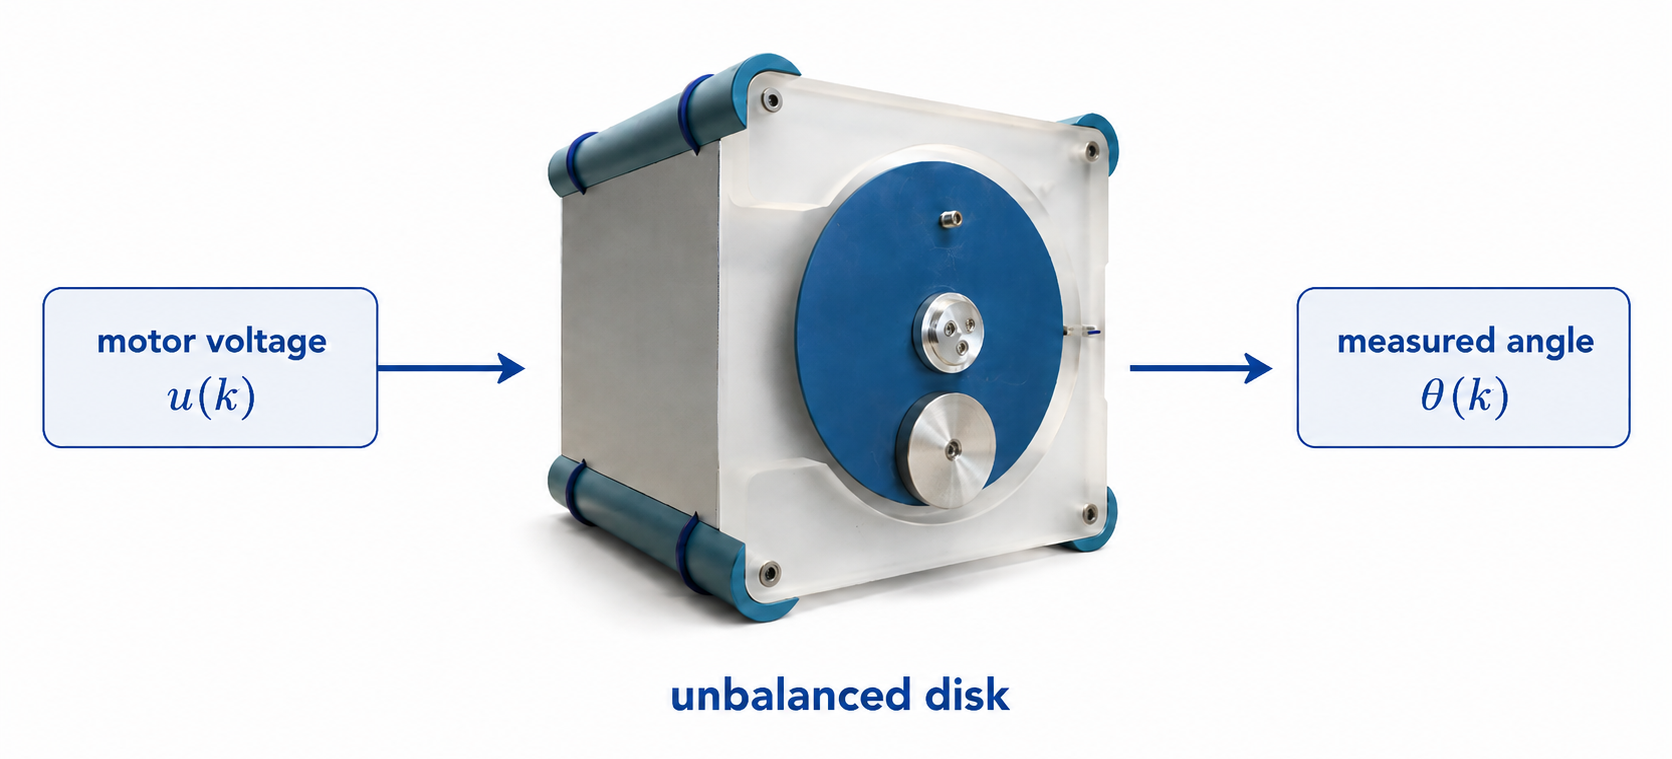
\includegraphics[width=\columnwidth]{figures/system_overview.png}}
\caption{Input-output view of the unbalanced disk system. The applied motor voltage \(u(k)\) is used as model input, and the measured disk angle \(\theta(k)\) is used as model output.}
\label{fig:system_overview}
\end{figure}

\subsection{Prediction and Simulation}

The models are evaluated using both prediction and simulation.
In prediction, the model uses measured past angles to predict the next angle.
In simulation, the model feeds back its own previous predictions to generate a full trajectory.
Simulation is harder because errors can accumulate over time, so both tasks are needed to judge the model properly \cite{course5sc28}.
The error was evaluated using the root mean squared error (RMSE):

\begin{equation}
\mathrm{RMSE} =
\sqrt{\frac{1}{N}\sum_{k=1}^{N}\left(\theta(k)-\hat{\theta}(k)\right)^2},
\end{equation}

where \(\theta(k)\) is the measured disk angle, \(\hat{\theta}(k)\) is the model output, and \(N\) is the number of evaluated samples.

\section{Artificial Neural Network Modelling}
\subsection{Method}

The ANN part required at least one simple ANN model and one more
advanced ANN architecture \cite{assignment5sc28}. Therefore, three
models were compared: a feedforward NARX ANN, a GRU, and an LSTM.

Since the system is dynamic, past inputs and outputs are needed. A
nonlinear autoregressive model with exogenous input (NARX) is written as

\begin{equation}
\begin{aligned}
\hat{\theta}(k)
=
f\big(&
\theta(k-1),\ldots,\theta(k-n_a),\\
&
u(k-1),\ldots,u(k-n_b)
\big),
\end{aligned}
\label{eq:ann_narx_general}
\end{equation}

where \(n_a\) and \(n_b\) are the output and input memory lengths. The
simple ANN approximates \(f(\cdot)\) with a feedforward network with one
hidden layer of 50 neurons, following the practical-session structure
\cite{course5sc28}. Both memory lengths were set to 15.
In prediction mode, the delayed angles in \eqref{eq:ann_narx_general}
are measured values. In simulation mode, the model must use its own
previous outputs instead of the measured previous angles. In other
words, simulation uses the same model structure as
\eqref{eq:ann_narx_general}, but replaces the measured delayed angles
\(\theta\) by the simulated delayed angles
\(\hat{\theta}_{\mathrm{sim}}\). This is why simulation is a stricter
test than one-step prediction: small errors can be fed back into the
model and affect later samples.

The GRU and LSTM use the same history length \(H=15\), but read it as an
ordered sequence of voltage-angle pairs instead of one flattened vector.
A recurrent network updates an internal state while reading this
sequence:

\begin{equation}
\begin{aligned}
\mathbf{h}_j
&=
g_{\mathrm{RNN}}(\mathbf{h}_{j-1}, [u(j),\theta(j)]),\\
\hat{\theta}(k)
&=
W_o\mathbf{h}_{k-1}+b_o .
\end{aligned}
\label{eq:ann_recurrent_state}
\end{equation}

The hidden state \(\mathbf{h}_j\) stores information from previous
samples. The GRU is simpler, while the LSTM has a more detailed memory
mechanism \cite{course5sc28,cho2014gru,hochreiter1997lstm}.
All models were trained using normalized data, mean squared error loss,
and the Adam optimizer \cite{kingma2014adam}. The known data were split
into 70\% training, 15\% validation, and 15\% test data. The complete
identification dataset contained 35000 measured samples, giving 24500
raw training samples, 5250 validation samples, and 5250 test samples.
Because the ANN inputs use past samples, the supervised training set was
slightly smaller: 24485 training examples for history length 15.

Seven ANN configurations were compared: one NARX ANN, one GRU, one final
LSTM, and four LSTM tuning runs. The LSTM tuning runs are shown in
Table~\ref{tab:lstm_tuning}.

\begin{table}[htbp]
\caption{LSTM tuning results on the held-out test split.}
\centering
\begin{tabular}{cccc}
\toprule
History & Hidden size & Prediction RMSE & Simulation RMSE \\
\midrule
10 & 20 & 0.458 deg & 2.433 deg \\
15 & 20 & 0.394 deg & 2.227 deg \\
15 & 40 & 0.267 deg & 2.384 deg \\
15 & 60 & 0.218 deg & 1.771 deg \\
\bottomrule
\end{tabular}
\label{tab:lstm_tuning}
\end{table}

History length 15 and hidden size 60 gave the best LSTM simulation
result. This architecture was then retrained with the NARX and GRU for
the final comparison. Since training is stochastic, the retrained LSTM
result in Table~\ref{tab:ann_results} differs slightly from the tuning
value.

\subsection{ANN Results}

Table~\ref{tab:ann_results} compares the simple NARX ANN, GRU, and
LSTM. The project files report errors in radians and degrees; the table
uses degrees for readability.

\begin{table}[htbp]
\caption{ANN results on the held-out test split.}
\centering
\begin{tabular}{lcc}
\toprule
Model & Prediction RMSE & Simulation RMSE \\
\midrule
Simple NARX ANN & 2.442 deg & 16.130 deg \\
Advanced GRU ANN & 0.202 deg & 2.031 deg \\
Advanced LSTM ANN & 0.235 deg & 1.893 deg \\
\bottomrule
\end{tabular}
\label{tab:ann_results}
\end{table}

Fig.~\ref{fig:ann_errors} shows the same comparison. The left plot uses a
logarithmic scale because the NARX simulation error is much larger; the
right plot zooms in on GRU and LSTM.

\begin{figure}[htbp]
\centerline{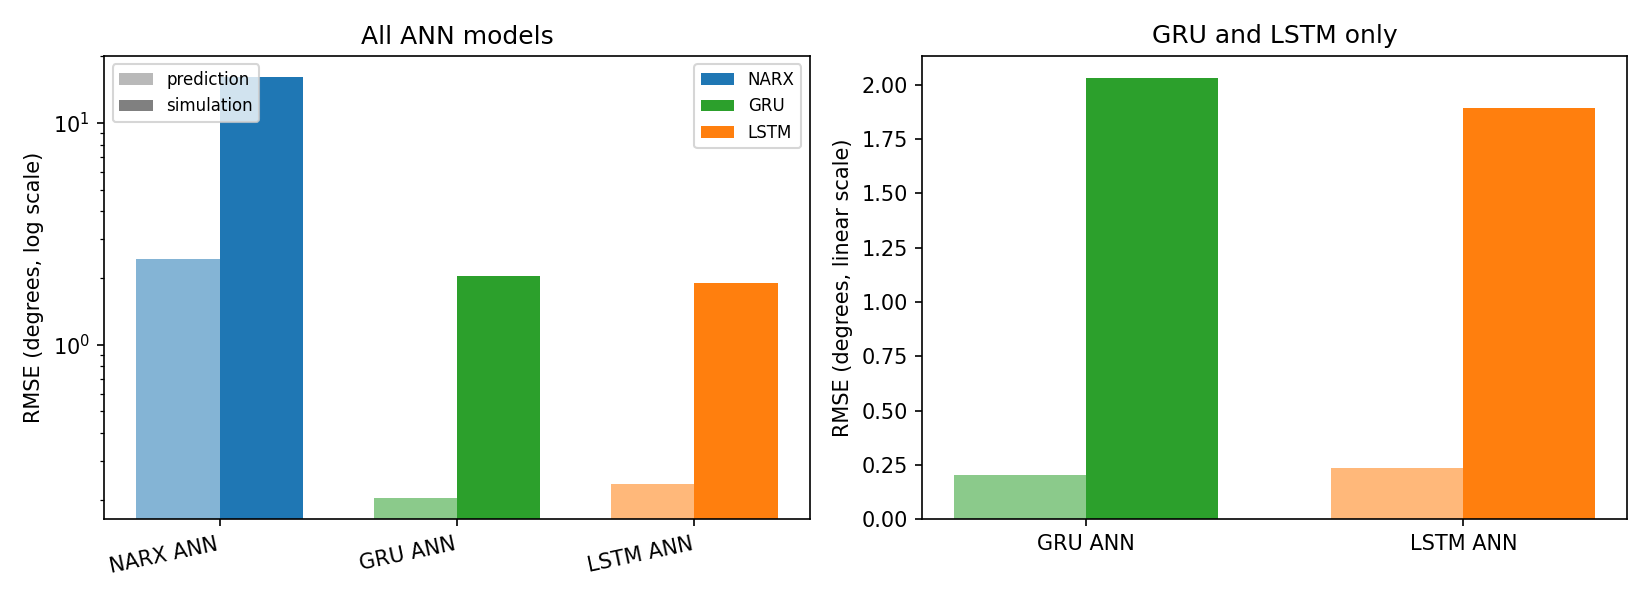
\includegraphics[width=\columnwidth]{figures/ann_three_model_comparison.png}}
\caption{Prediction and simulation RMSE for the three ANN models.}
\label{fig:ann_errors}
\end{figure}

Both recurrent models clearly outperformed the simple NARX ANN. The GRU
gave the best prediction result, while the LSTM gave the best simulation
result. This is reasonable because prediction uses measured past angles,
whereas simulation feeds the model's own predictions back into the
input.

Fig.~\ref{fig:ann_prediction} shows the prediction errors for the recurrent models.
This plot is used instead of only showing angle trajectories, because
the GRU and LSTM trajectories are very close to the measured angle.

\begin{figure}[htbp]
\centerline{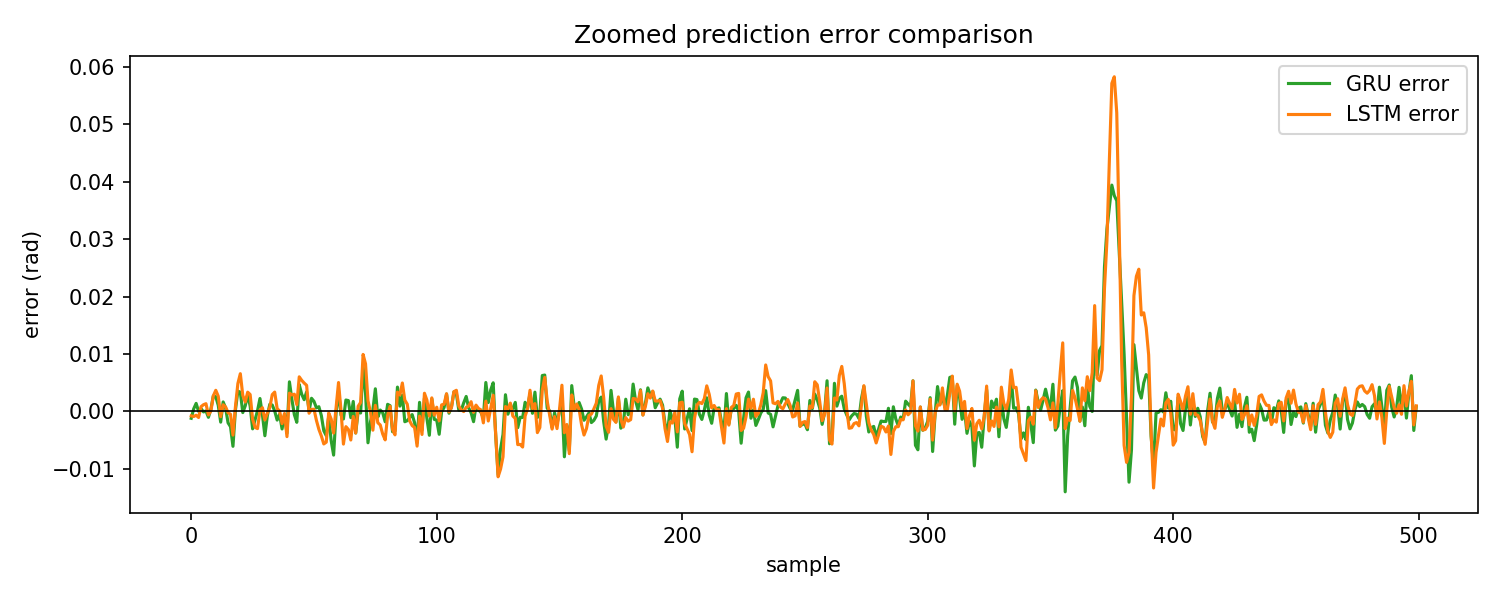
\includegraphics[width=\columnwidth]{figures/ann_prediction_error_zoom.png}}
\caption{Prediction error for the GRU and LSTM models.}
\label{fig:ann_prediction}
\end{figure}

Fig.~\ref{fig:ann_simulation} shows the simulation errors for the recurrent models.
This is the more important long-term comparison, because the model must
feed back its own previous predictions.

\begin{figure}[htbp]
\centerline{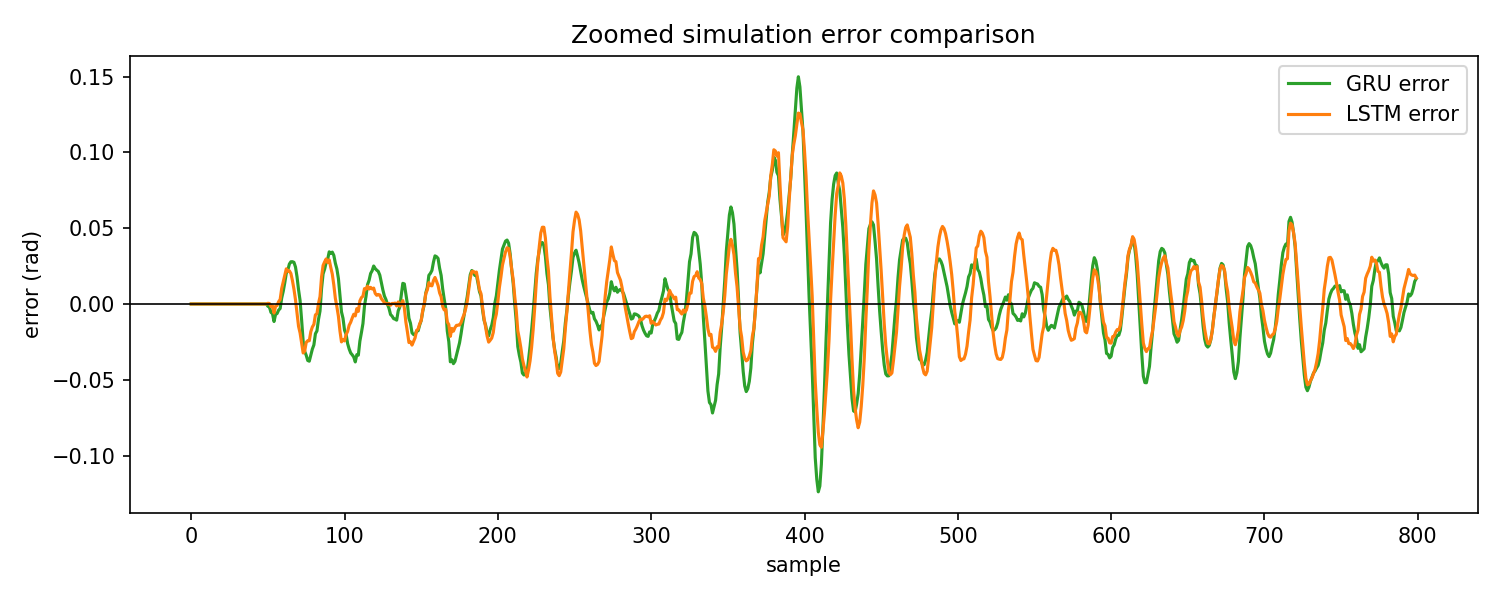
\includegraphics[width=\columnwidth]{figures/ann_simulation_error_zoom.png}}
\caption{Simulation error for the GRU and LSTM models.}
\label{fig:ann_simulation}
\end{figure}

\subsection{ANN Discussion}

The GRU was added to check whether the extra LSTM complexity was needed.
GRU is slightly better for prediction, but LSTM is better for simulation.
The main limitations are the small hyperparameter search, error
accumulation in simulation, and the fact that the ANN gives point
predictions without uncertainty estimates.


\section{GP Modelling Method}


\subsection{Method}

The GP part of the assignment required one nonlinear model structure to
be fitted and analysed using the measured motor voltage and disk angle
\cite{assignment5sc28}. The angular velocity was therefore not used.
A nonlinear autoregressive model with exogenous input (NARX) was
selected because the delayed input and output samples provide an
input--output representation of the system dynamics without requiring
an explicit state estimate.

The NARX regressor is defined as

\begin{equation}
\begin{aligned}
\mathbf{x}(k) =
\big[&
u(k-n_b),\ldots,u(k-1),\\
&
\theta(k-n_a),\ldots,\theta(k-1)
\big]^{\top},
\end{aligned}
\label{eq:gp_regressor}
\end{equation}

where \(n_a\) is the number of delayed angle samples and \(n_b\) is the
number of delayed voltage samples. Because the Mat\'ern-\(5/2\) kernel
is used with automatic relevance determination, each component of
\(\mathbf{x}(k)\) is assigned its own length scale, so the ordering of
the regressor entries does not affect the model. The ordering in
\eqref{eq:gp_regressor} is fixed to match the implementation, so that
the delayed angle \(\theta(k-1)\) occupies the last entry and is used
directly in the angle reconstruction \eqref{eq:gp_angle_reconstruction}.

Instead of predicting the absolute angle directly, the final model
predicts the angle increment

\begin{equation}
\Delta\theta(k)=\theta(k)-\theta(k-1).
\label{eq:gp_delta_target}
\end{equation}

The GP-NARX model is therefore written as

\begin{equation}
\Delta\theta(k)
=
f_{\mathrm{GP}}\!\left(\mathbf{x}(k)\right)+e(k),
\label{eq:gp_delta_model}
\end{equation}

and the predicted angle is reconstructed using

\begin{equation}
\hat{\theta}(k)
=
\theta(k-1)+\widehat{\Delta\theta}(k).
\label{eq:gp_angle_reconstruction}
\end{equation}

The delta-output formulation was used because the change in angle
between two consecutive samples is smaller and smoother than the
absolute angle. The GP therefore models the local system evolution
instead of the complete angle signal. In the experiments, this reduced
the recursive simulation error compared with direct angle prediction.

A Gaussian Process defines a probability distribution over possible
nonlinear functions \cite{course5sc28}. For the model in
\eqref{eq:gp_delta_model}, the unknown function is assigned the prior

\begin{equation}
f_{\mathrm{GP}}(\mathbf{x})
\sim
\mathcal{GP}\!\left(0,k(\mathbf{x},\mathbf{x}')\right),
\end{equation}

where \(k(\mathbf{x},\mathbf{x}')\) is the covariance kernel. Given the
training inputs \(\mathbf{X}\) and targets \(\mathbf{y}\), conditioning
this prior on the data yields a Gaussian predictive distribution
\cite{course5sc28}. The predictive mean at a new regressor
\(\mathbf{x}_{*}\) is

\begin{equation}
\hat{f}(\mathbf{x}_{*})
=
\mathbf{k}_{*}^{\top}
\left(
\mathbf{K}+\sigma_n^2\mathbf{I}
\right)^{-1}
\mathbf{y},
\label{eq:gp_mean}
\end{equation}

while the predictive variance is

\begin{equation}
\hat{\sigma}_{f}^{2}(\mathbf{x}_{*})
=
k(\mathbf{x}_{*},\mathbf{x}_{*})
-
\mathbf{k}_{*}^{\top}
\left(
\mathbf{K}+\sigma_n^2\mathbf{I}
\right)^{-1}
\mathbf{k}_{*}.
\label{eq:gp_variance}
\end{equation}

Equations \eqref{eq:gp_mean}--\eqref{eq:gp_variance} are the full GP
predictive mean and variance \cite{course5sc28}. The predictive mean is
used as the model output, while the predictive variance represents the
remaining model uncertainty. The predictive mean can equivalently be
written as

\begin{equation}
\hat{f}(\cdot)
=
\sum_i \hat{\alpha}_i\,k(\cdot,\mathbf{x}_i),
\qquad
\hat{\boldsymbol{\alpha}}
=
\left(\mathbf{K}+\sigma_n^2\mathbf{I}\right)^{-1}\mathbf{y}.
\label{eq:gp_kernel_expansion}
\end{equation}

This is the core GP estimator. The kernel hyperparameters (the ARD
length scales and the kernel variance) together with the Gaussian noise
variance \(\sigma_n^2\) were estimated from the training data by
minimizing the negative log marginal likelihood
\begin{equation}
\begin{aligned}
-\log p(\mathbf{y}\mid\mathbf{X},\boldsymbol{\eta})
={}& \tfrac{N}{2}\log 2\pi
+ \underbrace{\tfrac{1}{2}\mathbf{y}^{\top}\!\left(\mathbf{K}+\sigma_n^2\mathbf{I}\right)^{-1}\!\mathbf{y}}_{\text{data-fit term}}\\
&+ \underbrace{\tfrac{1}{2}\log\det\!\left(\mathbf{K}+\sigma_n^2\mathbf{I}\right)}_{\text{complexity term}}.
\end{aligned}
\label{eq:gp_marglik}
\end{equation}

which automatically trades off a data-fit term against a
model-complexity term \cite{course5sc28}. In the implementation this
objective was minimized with the L-BFGS-B optimizer using its analytic
gradient.

The regressors and target values were normalized before training.
After constructing the delayed regressors, the available records
contained \(24490\) training samples and \(10490\) validation samples.
The temporal order of the data was preserved, since random shuffling of
individual time samples would not provide a realistic free-run
simulation test.

Preliminary GP experiments compared several kernels using the same
initial direct-output NARX structure. These early tests were used only
to choose a reasonable kernel before the final sparse delta-output GP
was trained. The results are shown in
Table~\ref{tab:gp_kernel_comparison}.

\begin{table}[htbp]
\caption{Initial GP kernel comparison on the validation data.}
\centering
\begin{tabular}{lc}
\toprule
Kernel & Prediction RMSE \\
\midrule
RBF & 0.3583 deg \\
Mat\'ern-\(3/2\) & 0.2514 deg \\
Linear + RBF & 0.2515 deg \\
Mat\'ern-\(5/2\) & 0.2147 deg \\
\bottomrule
\end{tabular}
\label{tab:gp_kernel_comparison}
\end{table}

The Mat\'ern-\(5/2\) kernel gave the lowest validation prediction error
and was therefore selected. Compared with the RBF kernel, the
Mat\'ern-\(5/2\) kernel assumes less restrictive smoothness, which is
useful for modelling nonlinear mechanical dynamics containing friction
and rapidly changing local behaviour. Automatic relevance
determination was used, meaning that each delayed input and output
component had its own length scale.

The lag orders were then varied using

\begin{equation}
n_a\in\{5,8,10\},
\qquad
n_b\in\{5,8\}.
\label{eq:gp_lag_grid}
\end{equation}

In the preliminary lag-order tests, the setting \(n_a=10,n_b=5\)
gave the best first-round one-step prediction result, while the setting
\(n_a=10,n_b=8\) gave the best free-run simulation result among the
tested models. Since the assignment evaluates both prediction and
simulation, the latter configuration was selected. Ten delayed angle
samples provide sufficient output memory, while eight delayed voltage
samples capture the delayed influence of the motor input without making
the regressor unnecessarily large.

A full GP assigns one kernel slice \(k(\cdot,\mathbf{x}_i)\) and one
weight \(\hat{\alpha}_i\) to every training sample, so kernel-matrix
inversion scales as \(\mathcal{O}(N^3)\) and becomes prohibitive for
the \(N=24490\) training samples
\cite{course5sc28}. The full data set was therefore summarized by
\(M\ll N\) inducing points. The \texttt{SparseGPRegression} model in
GPy implements the variational (VFE) sparse approximation, in which the
inducing inputs \(\mathbf{Z}\) together with the kernel and noise
hyperparameters are jointly optimized by maximizing a variational lower
bound on the marginal likelihood \eqref{eq:gp_marglik}. The inducing
points were initialized using MiniBatch \(k\)-means clustering on the
normalized regressors, so that their initial locations covered the
regions with the largest data density. During training, the
inducing-point locations, kernel variance, ARD length scales, and
Gaussian noise variance were further optimized with L-BFGS-B.

Table~\ref{tab:gp_tuning} summarizes the main modelling steps.

\begin{table}[htbp]
\caption{Main GP model tuning steps on the validation data.}
\centering
\begin{tabular}{lcc}
\toprule
Model & Prediction RMSE & Simulation RMSE \\
\midrule
Direct-output GP-NARX & 0.1994 deg & 2.9658 deg \\
Delta-output GP-NARX & 0.1844 deg & 2.5333 deg \\
Sparse delta GP, \(M=150\) & 0.1698 deg & 1.5043 deg \\
Sparse delta GP, \(M=250\) & 0.1638 deg & 1.4615 deg \\
\bottomrule
\end{tabular}
\label{tab:gp_tuning}
\end{table}

The comparison shows that predicting the angle increment improved both
prediction and simulation. Introducing the sparse GP approximation
also allowed all available training samples to be used instead of a
small subset. Increasing the number of inducing points from
\(M=150\) to \(M=250\) gave a further reduction in both errors.
Therefore, \(M=250\) was selected as the final value. This value is
still much smaller than the number of training samples, while providing
the best simulation result among the tested sparse models.

The final model is consequently a sparse delta-output GP-NARX model
with a Mat\'ern-\(5/2\) ARD kernel, \(n_a=10\), \(n_b=8\), and
\(M=250\) inducing points. One-step prediction uses measured past
angles in the regressor, whereas free-run simulation recursively feeds
the previously simulated angles back into the model.


\subsection{GP Results}

Table~\ref{tab:gp_results} summarizes the validation performance of the
final sparse delta-output GP-NARX model. The errors are reported in both
radians and degrees. The final model used \(n_a=10\), \(n_b=8\), a
Mat\'ern-\(5/2\) ARD kernel, and \(M=250\) inducing points.

\begin{table}[htbp]
\caption{Validation results of the final sparse GP model.}
\centering
\begin{tabular}{lcc}
\toprule
Task & RMSE [rad] & RMSE [deg] \\
\midrule
One-step prediction & 0.002859 & 0.1638 \\
Free-run simulation & 0.025508 & 1.4615 \\
\bottomrule
\end{tabular}
\label{tab:gp_results}
\end{table}

The one-step prediction error is considerably smaller than the
simulation error. In the prediction task, the measured past angles are
used to construct the NARX regressor at every sample. Therefore, local
prediction errors do not propagate to later time steps. In the
simulation task, only the initial output history is measured. The GP
then recursively uses its own simulated outputs, so small modelling
errors accumulate over time.

The final simulation normalized root mean squared error was

\begin{equation}
\mathrm{NRMS}_{\mathrm{sim}} = 5.04\%.
\end{equation}

Fig.~\ref{fig:gp_simulation} compares the measured validation output
with the free-run simulation of the final sparse GP model.

\begin{figure}[htbp]
\centerline{
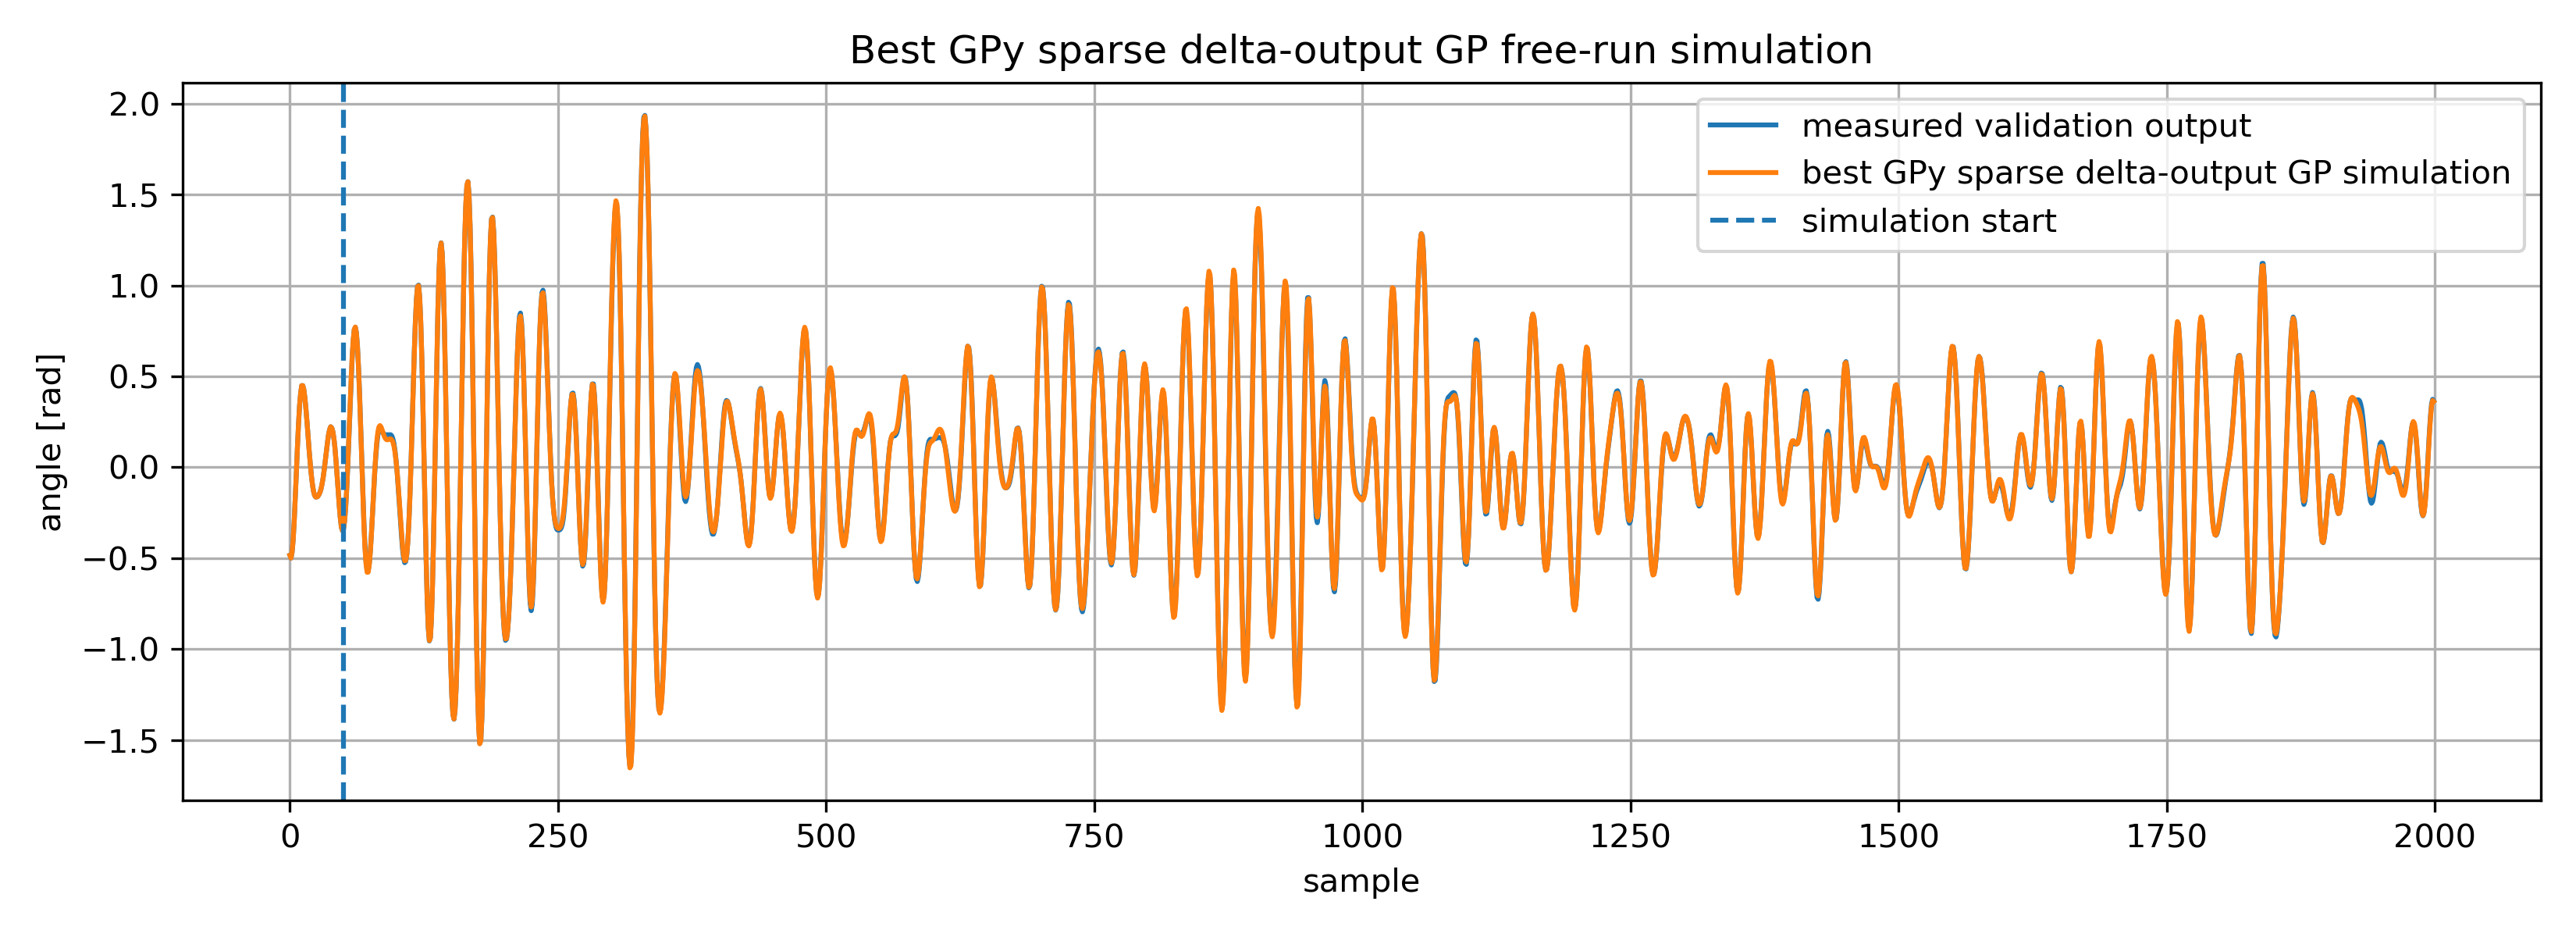
\includegraphics[width=\columnwidth]
{figures/gp_validation_simulation.png}
}
\caption{Measured validation angle and free-run simulation of the final
sparse delta-output GP-NARX model.}
\label{fig:gp_simulation}
\end{figure}

The simulated angle follows the measured output closely over most of
the validation interval. The model reproduces both the oscillation
frequency and the main amplitude variations. This indicates that the
selected delayed angle and voltage samples contain sufficient
information to represent the dominant input--output dynamics of the
disk.

The simulation error is shown in
Fig.~\ref{fig:gp_simulation_error}.

\begin{figure}[htbp]
\centerline{
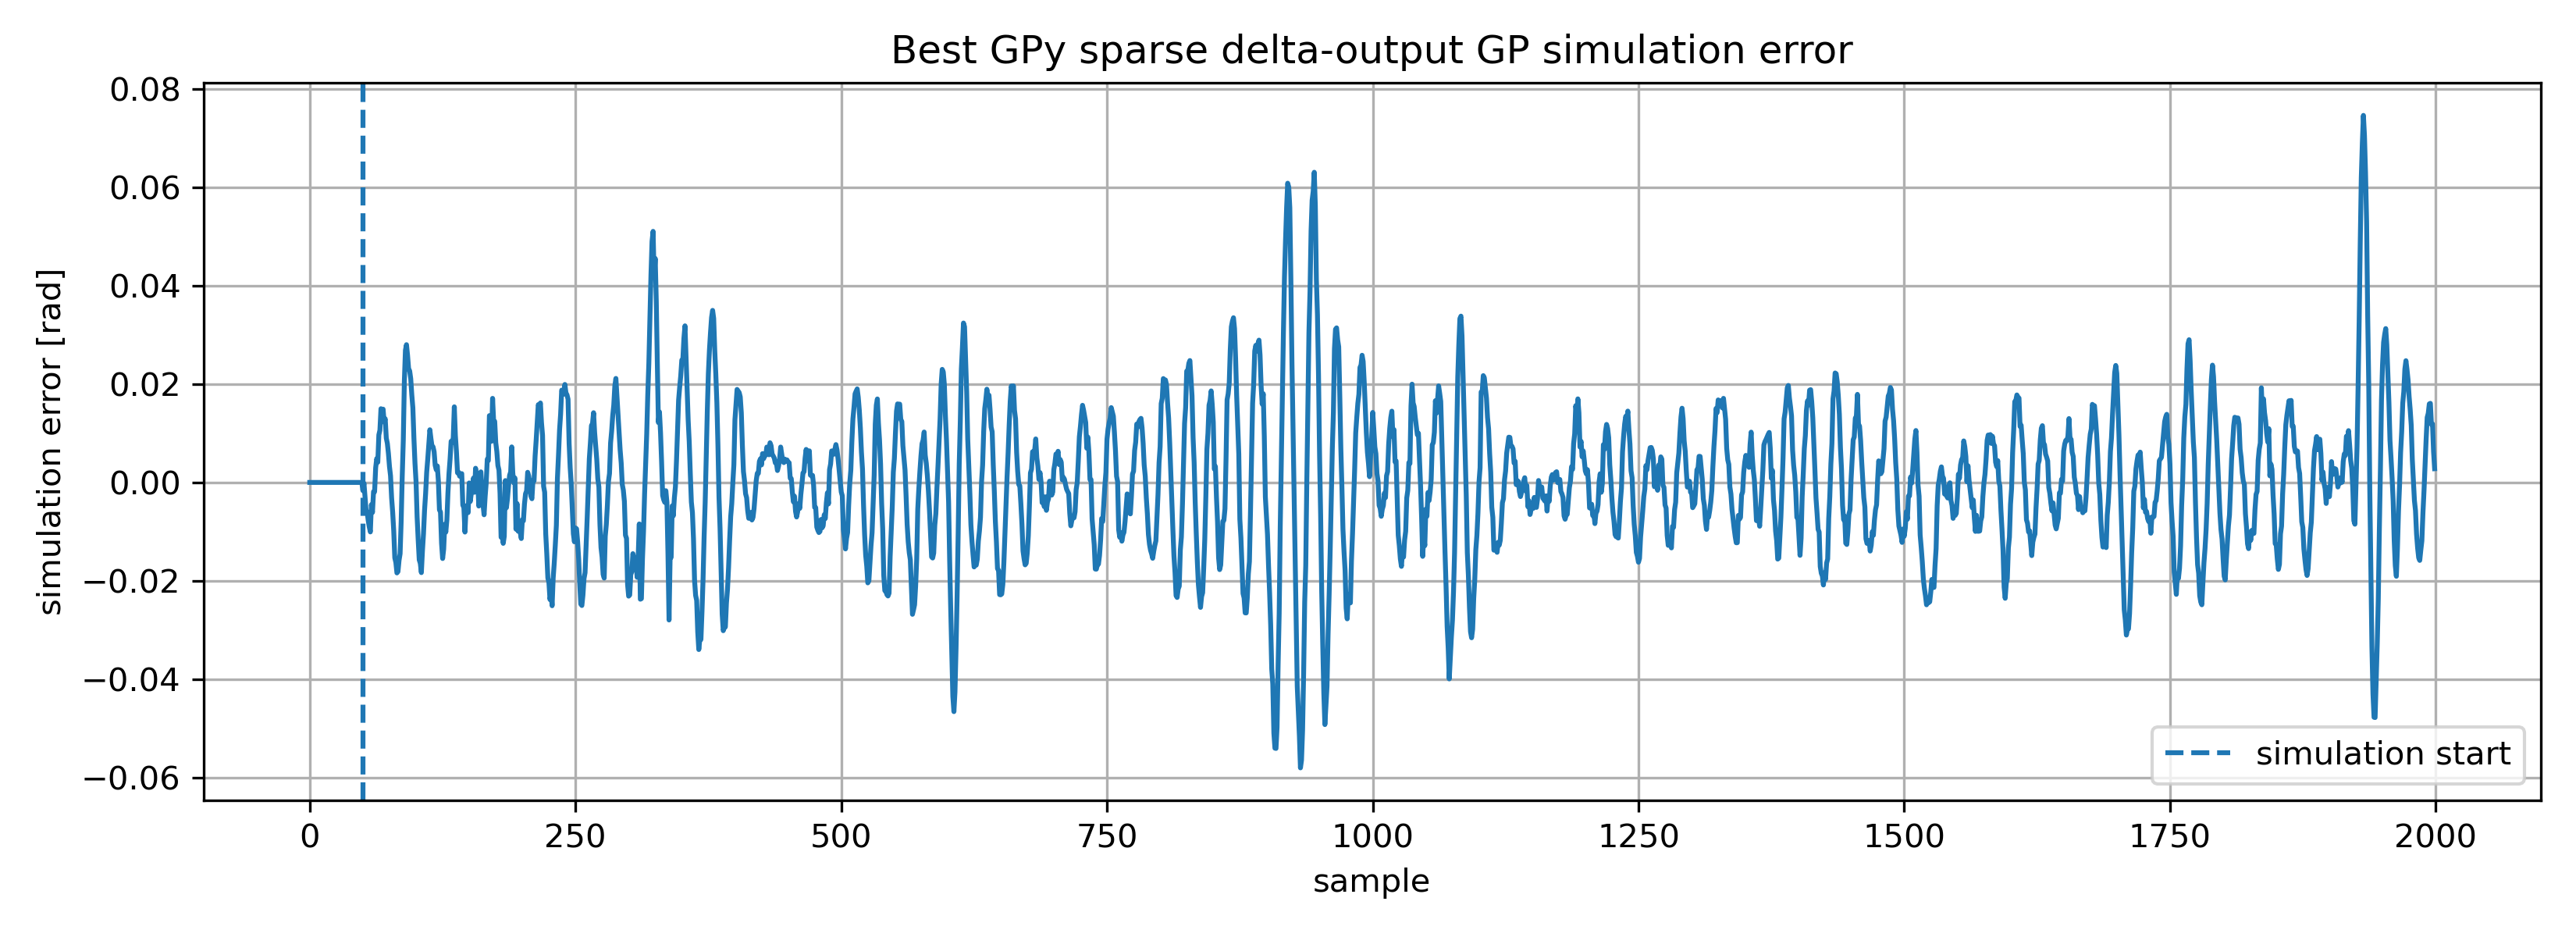
\includegraphics[width=\columnwidth]
{figures/gp_validation_simulation_error.png}
}
\caption{Free-run simulation error of the final sparse delta-output GP
model.}
\label{fig:gp_simulation_error}
\end{figure}

The simulation error remains close to zero for most samples. Larger
error peaks occur mainly during intervals with fast angle changes and
large oscillation amplitudes. These regions are more difficult because
a small error in the predicted angle increment also changes the
regressor used in the next simulation step. The resulting mismatch can
temporarily increase before the simulated trajectory returns close to
the measured trajectory.

The improvement obtained during the modelling procedure can also be
seen from the final results. The initial direct-output GP model had a
simulation RMSE of \(2.9658\) deg. Changing the target to the angle
increment reduced this value to \(2.5333\) deg. The sparse GP with
\(M=150\) inducing points further reduced the simulation RMSE to
\(1.5043\) deg, while increasing the number of inducing points to
\(M=250\) resulted in the final value of \(1.4615\) deg.


\subsection{GP Uncertainty and Optimized Hyperparameters}

Unlike a deterministic regressor, the GP also returns the predictive
variance \eqref{eq:gp_variance}, which provides a direct characterization
of the remaining model uncertainty and the associated \(95\%\)
confidence bound \cite{course5sc28}. The hyperparameters obtained by
minimizing the negative log marginal likelihood \eqref{eq:gp_marglik}
are summarized in Table~\ref{tab:gp_hyperparameters}.

\begin{table}[htbp]
\caption{Optimized hyperparameters of the final sparse GP model
(normalized \(\Delta\theta\) output units).}
\centering
\begin{tabular}{lc}
\toprule
Hyperparameter & Value \\
\midrule
Kernel variance \(\sigma_f^2\)   & \(0.674\) \\
Noise variance \(\sigma_n^2\)    & \(5.15\times 10^{-4}\) \\
ARD length scales                & \(18\) (one per regressor) \\
Inducing points \(M\)            & \(250\) \\
\bottomrule
\end{tabular}
\label{tab:gp_hyperparameters}
\end{table}

The number of ARD length scales is

\begin{equation}
n_a+n_b=18,
\end{equation}

confirming that each delayed angle and voltage sample receives its own length scale.
The very small estimated noise variance shows that the
marginal-likelihood fit attributes almost all of the normalized output
variation to the latent function rather than to measurement noise, i.e.\
a high signal-to-noise fit. This is consistent with the large data-fit
term in \eqref{eq:gp_marglik} and with the small one-step prediction
error in Table~\ref{tab:gp_results}.

The predictive variance \eqref{eq:gp_variance} is, however, the
\emph{one-step} posterior uncertainty evaluated at a deterministic
input. In free-run simulation the regressor itself contains previously
simulated, and therefore uncertain, angles. The implemented simulation
propagates only the predictive mean and feeds it back into the
regressor, so the reported confidence bound is exact for one-step
prediction but underestimates the true simulation uncertainty.
Propagating the full distribution would require evaluating the GP at an
uncertain (Gaussian) input, for example through moment matching
\cite{course5sc28}. This was considered out of scope here, since the
identification benchmark only requires the simulated mean trajectory.


\subsection{GP Discussion}

The final sparse delta-output GP-NARX model gave a one-step prediction
RMSE of \(0.1638\) deg and a free-run simulation RMSE of \(1.4615\) deg.
The larger simulation error is expected because prediction uses measured
past angles at every time step, while simulation recursively feeds the
model's own outputs back into the NARX regressor. Therefore, small local
errors can accumulate during simulation.

The Mat\'ern-\(5/2\) kernel was selected because it gave the best
validation prediction result among the tested kernels. It is less
restrictive than the RBF kernel with respect to function smoothness,
which makes it suitable for mechanical dynamics containing friction and
other locally varying nonlinear effects. The use of automatic relevance
determination also allowed every delayed voltage and angle component to
have a separate length scale. Large length scales indicate that the
corresponding regressor has a relatively small local influence, while
smaller length scales indicate a stronger sensitivity of the GP output.

The delta-output formulation improved both prediction and simulation
compared with direct angle prediction. Instead of learning the complete
angle value, the GP learns the smaller change between two consecutive
samples. This provides a more local representation of the dynamics and
reduces the variation of the regression target. However, recursive
simulation can still drift because an error in one predicted increment
changes the delayed angle values used in the following regressors.

The sparse GP approximation was necessary because a full GP scales
cubically with the number of training samples \cite{course5sc28}.
Using inducing points made it possible to train the model using the full
available training set. The inducing points were initialized using
MiniBatch \(k\)-means clustering, so that they initially represented
regions with a high density of regressors. Their locations and the GP
hyperparameters were then jointly optimized during training by
maximizing the variational bound on the marginal likelihood.

Increasing the number of inducing points from \(M=150\) to \(M=250\)
improved the prediction RMSE from \(0.1698\) deg to \(0.1638\) deg and
the simulation RMSE from \(1.5043\) deg to \(1.4615\) deg. The
improvement was relatively small, but \(M=250\) was selected because it
gave the best simulation result among the tested sparse models.
Simulation performance was given more weight in the final selection
because it evaluates whether the identified model can reproduce the
system dynamics recursively rather than only predict one sample ahead.

The selected lag orders \(n_a=10\) and \(n_b=8\) also represent a
trade-off. A larger number of delayed samples provides more information
about the system memory, but it also increases the regressor dimension
and the number of GP hyperparameters. Among the tested configurations,
this setting gave the best simulation performance without further
increasing the model dimension.

The main limitation is that only a finite set of kernels, lag orders,
and inducing-point counts was tested. A better configuration may
therefore still exist. In addition, the GP is reliable mainly in regions
that are sufficiently represented by the identification data. Since a
kernel model generally interpolates better than it extrapolates, the
prediction uncertainty and error may increase when the model is
evaluated outside the operating range of the training data. As discussed
above, the predictive variance also quantifies this growing uncertainty,
although in free-run simulation only the mean was propagated.

Finally, the true measured outputs for the hidden benchmark tests were
not available during development. Consequently, the final hidden
prediction and simulation files could only be checked for the required
format and dimensions before submission. Their actual performance will
be evaluated by the course staff.



\section{Policy Learning for Swing-Up}


The objective of the control part is to learn policies that swing up the
unbalanced disk from the stable downward equilibrium and stabilize it around
the unstable upright position \cite{assignment5sc28,course5sc28}. The input is the motor voltage and is constrained
by
\begin{equation}
    u_k \in [-3,3]~\mathrm{V}.
\label{eq:policy_voltage_limit}
\end{equation}
The disk angle $\theta$ and angular velocity $\omega$ are used as full state
feedback. The downward position is defined as $\theta=0$, while the upright
target corresponds to $\theta=\pi$. Since the angle is periodic, the upright
error is evaluated using the wrapped angle error
\begin{equation}
    e_{\theta,k}=\mathrm{wrap}(\theta_k-\pi),
\label{eq:policy_upright_error}
\end{equation}
so that both $\theta=\pi$ and $\theta=-\pi$ represent the same physical upright
configuration.

Two learning-based controllers are considered. The first one is a Deep
Q-Network (DQN) controller, which represents the Q-learning-based part of the
assignment. It learns a discrete-action voltage policy from simulator
interaction by approximating the action-value function with a neural network
\cite{course5sc28,watkins1992qlearning,mnih2015dqn}.
The second controller is a hybrid energy-pumping and RBF-based policy
improvement method. In this approach, an energy-pumping law is used for the
global swing-up phase, while an RBF policy initialized from local PD supervision
is used for stabilization near the upright position and further improved by
simulator-based optimization \cite{course5sc28,broomhead1988rbf}.

The controllers are evaluated using rollout-based metrics, including final and
last-window wrapped angle error, upright ratio, input saturation ratio, and
multi-seed success rate. These metrics assess not only whether the disk reaches
the upright position, but also whether it remains stable there without excessive
voltage saturation. The following sections present the DQN controller, the
hybrid RBF controller, and their comparison.



\subsection{Control Objective and Evaluation Metrics}

The control objective is to swing up the disk from the downward stable position
to the upright unstable equilibrium and keep it stabilized around that position.
For policy learning, full state feedback is allowed, so the controller uses
\begin{equation}
    x_k =
    \begin{bmatrix}
        \theta_k \\
        \omega_k
    \end{bmatrix},
\label{eq:policy_full_state}
\end{equation}
where $\theta_k$ is the measured disk angle and $\omega_k$ is the angular
velocity. The motor voltage is constrained by
\begin{equation}
    u_k \in [-3,3]~\mathrm{V}.
\label{eq:policy_input_constraint}
\end{equation}

Since the disk angle is periodic, the upright error is defined as the wrapped
angle error
\begin{equation}
    e_{\theta,k} = \mathrm{wrap}(\theta_k-\pi),
\label{eq:policy_wrapped_error}
\end{equation}
so that both $\theta=\pi$ and $\theta=-\pi$ correspond to the same physical
upright configuration. A successful controller should make
$|e_{\theta,k}|$ small and reduce $|\omega_k|$ after the disk reaches the
upright region.

The controllers are evaluated using rollout-based metrics, including the final
wrapped angle error, the minimum absolute error, the mean absolute error over
the last $N_w=100$ time steps, the last-window angular velocity, the upright
ratio, and the input saturation ratio. The upright ratio measures how long the
disk remains close to the target, while the saturation ratio measures how often
the input reaches the voltage limits. For multi-seed robustness evaluation, a
rollout is considered successful if
\begin{equation}
\begin{aligned}
    e_{\mathrm{last}} < 0.10
    \quad \mathrm{and} \quad
    r_{\mathrm{upright}} > 0.70.
\end{aligned}
\label{eq:policy_success_condition}
\end{equation}
The success rate is then computed as the fraction of successful rollouts over
all tested seeds.



\subsubsection{Method and State-Action Representation}

The first learning-based controller was implemented using Deep Q-Network (DQN)
learning, which represents the Q-learning-based method in this project
\cite{watkins1992qlearning,mnih2015dqn}. Since
the disk angle and angular velocity are continuous variables, a tabular
Q-function is not practical. Therefore, a neural network was used to approximate
the action-value function \(Q(s_k,u_k)\). After training, the controller applies
the greedy action
\begin{equation}
    u_k = \arg\max_{u \in \mathcal{U}} Q(s_k,u).
\label{eq:dqn_greedy_action}
\end{equation}

The DQN state was defined as
\begin{equation}
    s_k =
    \begin{bmatrix}
        \sin\theta_k \\
        \cos\theta_k \\
        \omega_k/10
    \end{bmatrix}.
\label{eq:dqn_state}
\end{equation}
The sine-cosine representation avoids the discontinuity of the periodic angle
at \(\theta=\pm\pi\), while the angular velocity is scaled to keep all state
components in a similar numerical range.

Because DQN is a discrete-action method, the motor voltage was discretized as
\begin{equation}
    \mathcal{U} =
    \{-3,-2,-1,0,1,2,3\}~\mathrm{V}.
\label{eq:dqn_action_set}
\end{equation}
This action set satisfies the voltage constraint by construction. The DQN
network takes \(s_k\) as input and outputs one Q-value for each admissible
voltage action. During evaluation, the action with the highest Q-value is
applied to the simulator. The main advantage of this design is that it enables
Q-learning on the continuous-state unbalanced disk system, while the main
limitation is that the resulting voltage input is discrete and may be less
smooth than a continuous-action policy.


\subsubsection{Reward Function and Training Setup}

The DQN reward was shaped to encourage both energy injection during the
swing-up phase and stabilization near the upright position. A sparse reward
based only on the final upright condition would make exploration difficult, so
the reward was constructed from height, upright, bonus, angular-velocity, and
input-effort terms:
\begin{equation}
\begin{aligned}
    r_k =
    r_{\mathrm{height},k}
    + r_{\mathrm{upright},k}
    + r_{\mathrm{bonus},k}
    - r_{\omega,k}
    - r_{u,k}.
\end{aligned}
\label{eq:dqn_reward}
\end{equation}
The height term encourages the disk to move away from the downward equilibrium,
while the upright and bonus terms reward small wrapped error near the target.
The angular-velocity and input penalties reduce excessive oscillation and
unnecessary control effort. The stabilization-related terms use
\begin{equation}
    e_{\theta,k}=\mathrm{wrap}(\theta_k-\pi),
\label{eq:dqn_reward_error}
\end{equation}
so that both \(\theta=\pi\) and \(\theta=-\pi\) are treated as the same upright
configuration.

Training was performed in the official unbalanced-disk simulator using an
\(\epsilon\)-greedy exploration strategy \cite{course5sc28}. The exploration probability was
gradually reduced during training, so that the agent first explored different
swing-up behaviors and later relied more on the learned Q-function. Experience
replay and a target network were used to improve the stability of the DQN
updates \cite{mnih2015dqn}. The best checkpoint was selected based on the evaluation rollout
performance and was later tested using the greedy policy without exploration.

\begin{figure}[H]
    \centering
    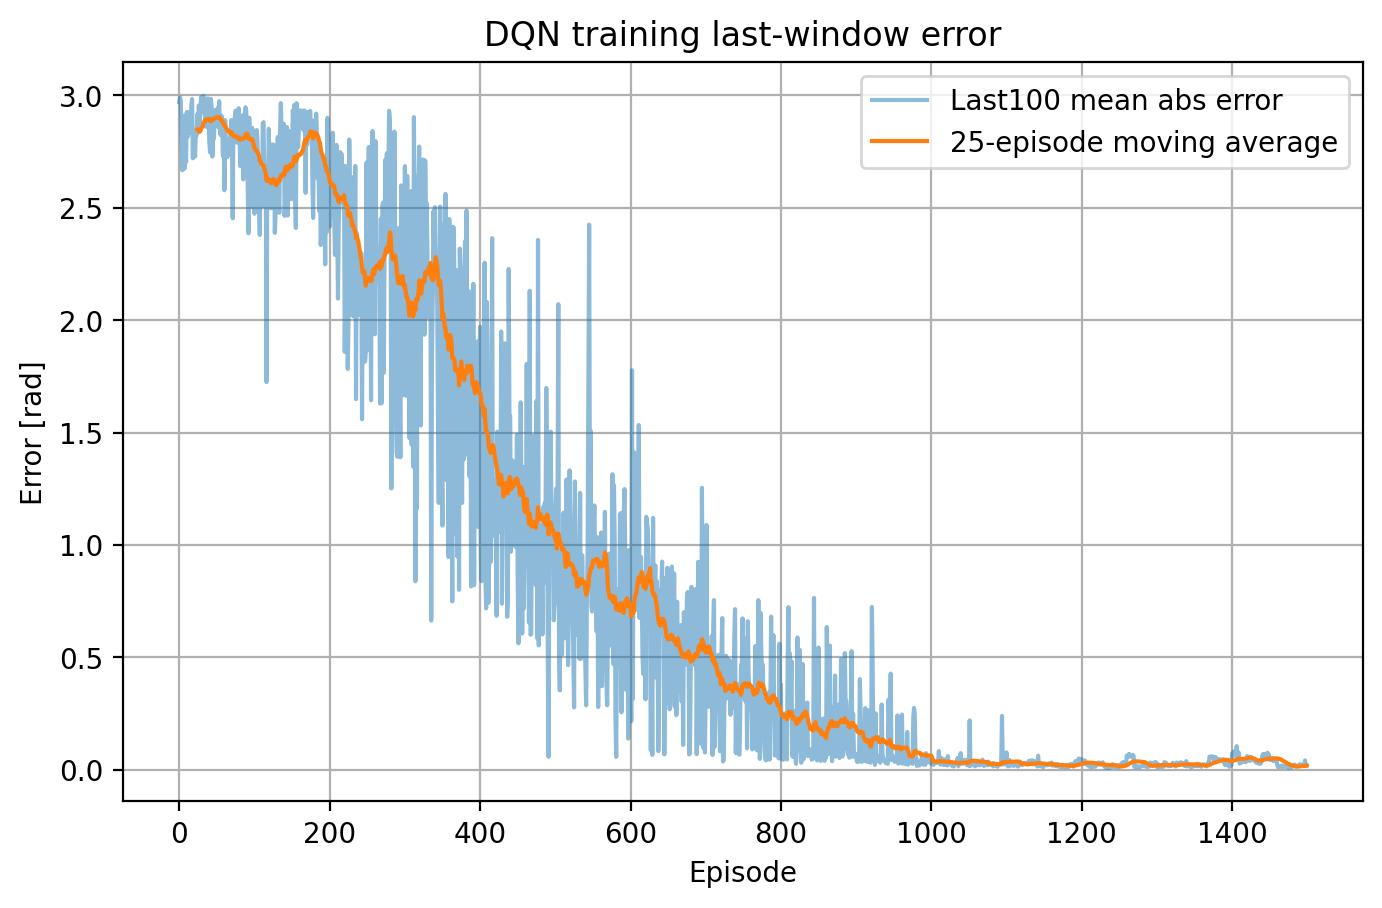
\includegraphics[width=0.85\linewidth]{figures/dqn_training_last100_error.png}
    \caption{Last-window mean absolute angle error during DQN training. The
    decreasing error indicates that the learned policy gradually improves its
    final upright stabilization performance.}
    \label{fig:dqn_training_error}
\end{figure}

As shown in Fig.~\ref{fig:dqn_training_error}, the training error decreases as
the agent collects more simulator experience. This confirms that the learned
Q-function gradually improves from random exploratory behavior to an effective
swing-up and stabilization policy.


\subsubsection{Simulation Results}

After training, the best DQN checkpoint was evaluated using the greedy policy
without exploration,
\begin{equation}
    u_k = \arg\max_{u \in \mathcal{U}} Q(s_k,u).
\label{eq:dqn_eval_action}
\end{equation}
Figure~\ref{fig:dqn_greedy} shows that the wrapped angle error decreases after
the swing-up phase and remains close to zero near the end of the rollout. This
confirms that the learned DQN policy can drive the disk to the upright
configuration and stabilize it there in simulation.

\begin{figure}[H]
    \centering
    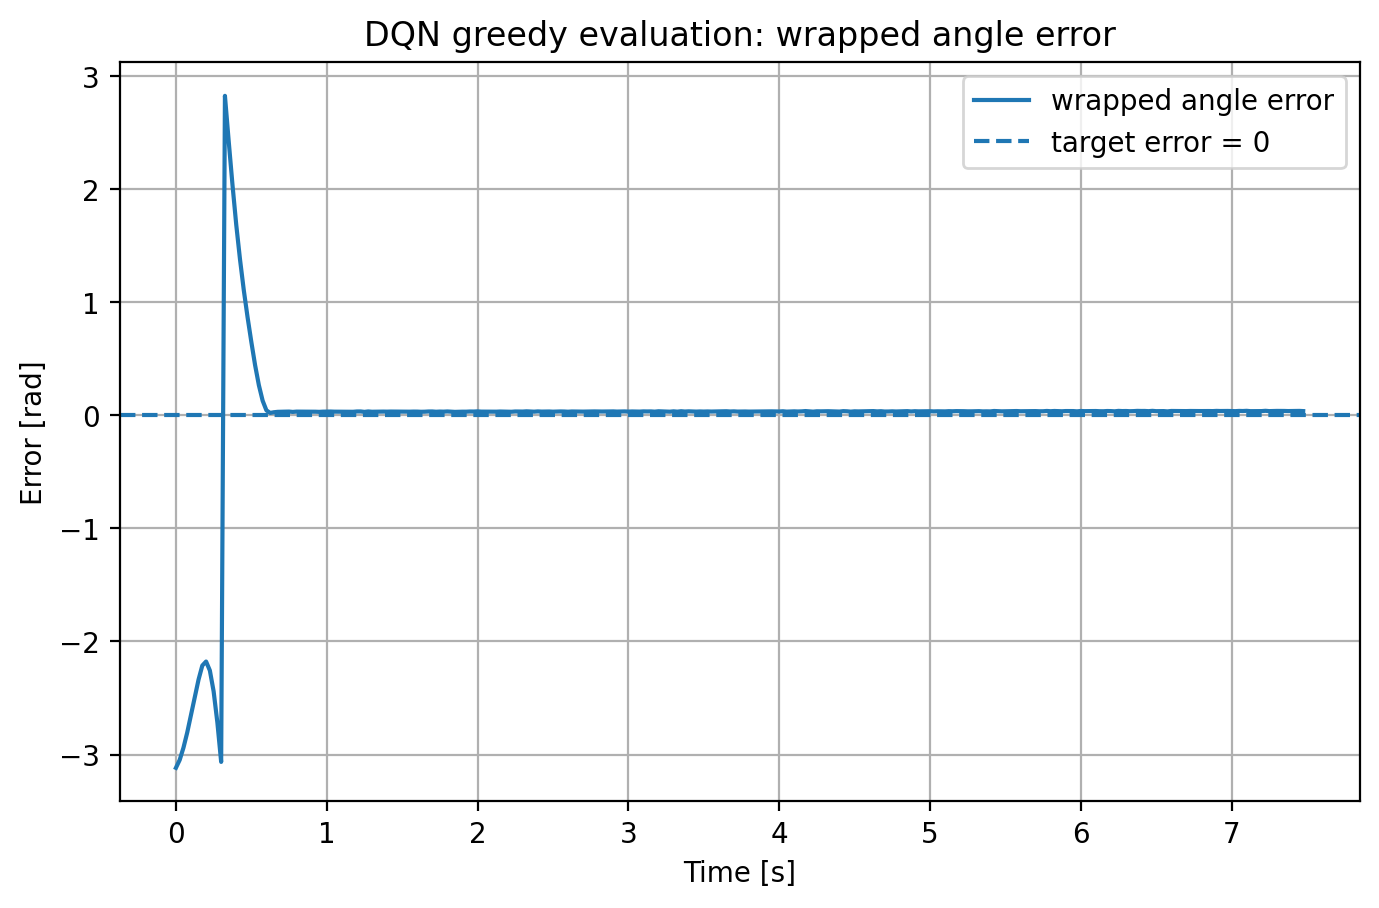
\includegraphics[width=0.85\linewidth]{figures/dqn_eval_best_error.png}
    \caption{Wrapped angle error of the greedy DQN policy. The error converges
    close to zero after the swing-up phase.}
    \label{fig:dqn_greedy}
\end{figure}

The best policy was further evaluated over 20 random simulation seeds. The
results in Table~\ref{tab:dqn_results} show that the DQN achieved a success
rate of $1.000$. The last-window mean absolute error was $0.0317$ rad and the
last-window mean absolute angular velocity was $0.0014$ rad/s, indicating that
the disk was stabilized near the upright position rather than only passing
through it.

\begin{table}[htbp]
    \caption{Multi-seed evaluation performance of the best DQN policy.}
    \centering
    \begin{tabular}{lc}
        \toprule
        Metric & Value \\
        \midrule
        Evaluation seeds & 20 \\
        Success rate & 1.000 \\
        Final error [rad] & $0.0326 \pm 0.0068$ \\
        Min. abs. error [rad] & $0.0198 \pm 0.0026$ \\
        Mean abs. error [rad] & $0.1879 \pm 0.0054$ \\
        Last-window error [rad] & $0.0317 \pm 0.0062$ \\
        Last-window $|\omega|$ [rad/s] & $0.0014 \pm 0.0014$ \\
        Upright ratio & $0.9233 \pm 0.0000$ \\
        Saturation ratio & $0.0733 \pm 0.0000$ \\
        Return & $1385.6200 \pm 1.5405$ \\
        \bottomrule
    \end{tabular}
    \label{tab:dqn_results}
\end{table}

Overall, the DQN controller successfully solved the swing-up and stabilization
task in simulation. Its main advantage is that it learns the control policy
directly from interaction data without an explicit analytical swing-up law.
However, the controller uses a discrete voltage action set, so the resulting
input may be less smooth than that of a continuous policy.



\subsection{Hybrid Energy-Pumping and RBF Policy Improvement}

\subsubsection{Design Motivation and Hybrid Policy Structure}

The second controller was developed as a hybrid energy-pumping and RBF-based
policy improvement method. In contrast to the DQN controller, which learns a
value function from simulator interaction, this approach combines physical
insight for the swing-up phase with a learned nonlinear local stabilizer near
the upright position \cite{course5sc28,broomhead1988rbf}. This controller is used as the model-internalization or
policy-improvement branch of the study.

A direct global RBF imitation policy was first tested using teacher data from
an energy-pumping and local PD controller. However, closed-loop simulations
showed that the global RBF policy was not robust: it could sometimes pass
through the upright region, but often failed to stabilize the disk or produced
nearly saturated inputs. Therefore, the task was separated into a global
swing-up part and a local stabilization part.

The resulting hybrid policy is
\begin{equation}
\begin{aligned}
    u_k =
    \begin{cases}
        u_{\mathrm{energy}}(\theta_k,\omega_k),
        & |e_{\theta,k}| \geq \epsilon, \\[2mm]
        g_{\mathrm{RBF}}\pi_{\mathrm{RBF}}(x_k),
        & |e_{\theta,k}| < \epsilon,
    \end{cases}
\end{aligned}
\label{eq:hybrid_policy}
\end{equation}
where \(e_{\theta,k}=\mathrm{wrap}(\theta_k-\pi)\), \(\epsilon\) is the
switching threshold, and \(g_{\mathrm{RBF}}\) is the local stabilizer gain. The
energy-pumping controller injects energy when the disk is far from the upright
position, while the RBF policy is only used near the target region.

The RBF stabilizer uses the local state
\begin{equation}
    x_k =
    \begin{bmatrix}
        e_{\theta,k} \\
        \omega_k
    \end{bmatrix}
\label{eq:hybrid_local_state}
\end{equation}
and is written as the saturated feedback law
\begin{equation}
    \pi_{\mathrm{RBF}}(x_k)
    =
    u_{\max}\tanh\!\left(\Phi(x_k)w\right),
\label{eq:rbf_policy}
\end{equation}
with \(u_{\max}=3\) V. The hyperbolic tangent bounds the RBF output, and the
final input is clipped to satisfy \(u_k\in[-3,3]\) V. This structure reduces the
learning difficulty because the RBF policy only needs to learn local upright
stabilization, while the analytical energy-pumping law handles the global
swing-up motion.


\subsubsection{RBF Local Stabilizer Initialization}

After selecting the hybrid structure, the RBF component was initialized as a
local stabilizer around the upright equilibrium. Instead of using complete
swing-up teacher trajectories, a local supervision dataset was generated from a
PD controller, because the RBF policy is only active near the upright position.
The local state was defined as
\begin{equation}
    x =
    \begin{bmatrix}
        e_\theta \\
        \omega
    \end{bmatrix},
\label{eq:rbf_training_state}
\end{equation}
and the supervision grid covered
\begin{equation}
\begin{aligned}
    e_\theta \in [-0.6,0.6],
    \qquad
    \omega \in [-8,8].
\end{aligned}
\label{eq:rbf_training_grid}
\end{equation}
For each grid point, the target input was computed using
\begin{equation}
\begin{aligned}
    u_{\mathrm{PD}} = -K_p e_\theta - K_d \omega,
    \qquad
    K_p=10.0,\quad K_d=1.5,
\end{aligned}
\label{eq:rbf_pd_target}
\end{equation}
and clipped to the admissible range \([-3,3]\) V.

The RBF policy was trained to reproduce this local PD behavior using the
saturated form
\begin{equation}
    \pi_{\mathrm{RBF}}(x)
    =
    u_{\max}\tanh\!\left(\Phi(x)w\right).
\label{eq:rbf_saturated_policy}
\end{equation}
The final local stabilizer used 121 RBF basis functions and 122 trainable
parameters including the bias term. On the local supervision grid, the mean
absolute input error was
\begin{equation}
    \mathrm{MAE}_u = 0.0571~\mathrm{V},
\label{eq:rbf_mae}
\end{equation}
which indicates that the RBF policy accurately approximates the desired local
PD stabilizing action.

The initialized RBF stabilizer was then combined with the analytical
energy-pumping controller. The initial switching threshold was set to
\(\epsilon=0.45\) rad. As shown in Fig.~\ref{fig:hybrid_initial_angle}, the
initialized hybrid controller successfully swung up the disk and stabilized it
near the upright configuration in simulation. This provided a suitable starting
point for the following simulator-based policy improvement step.

\begin{figure}[H]
    \centering
    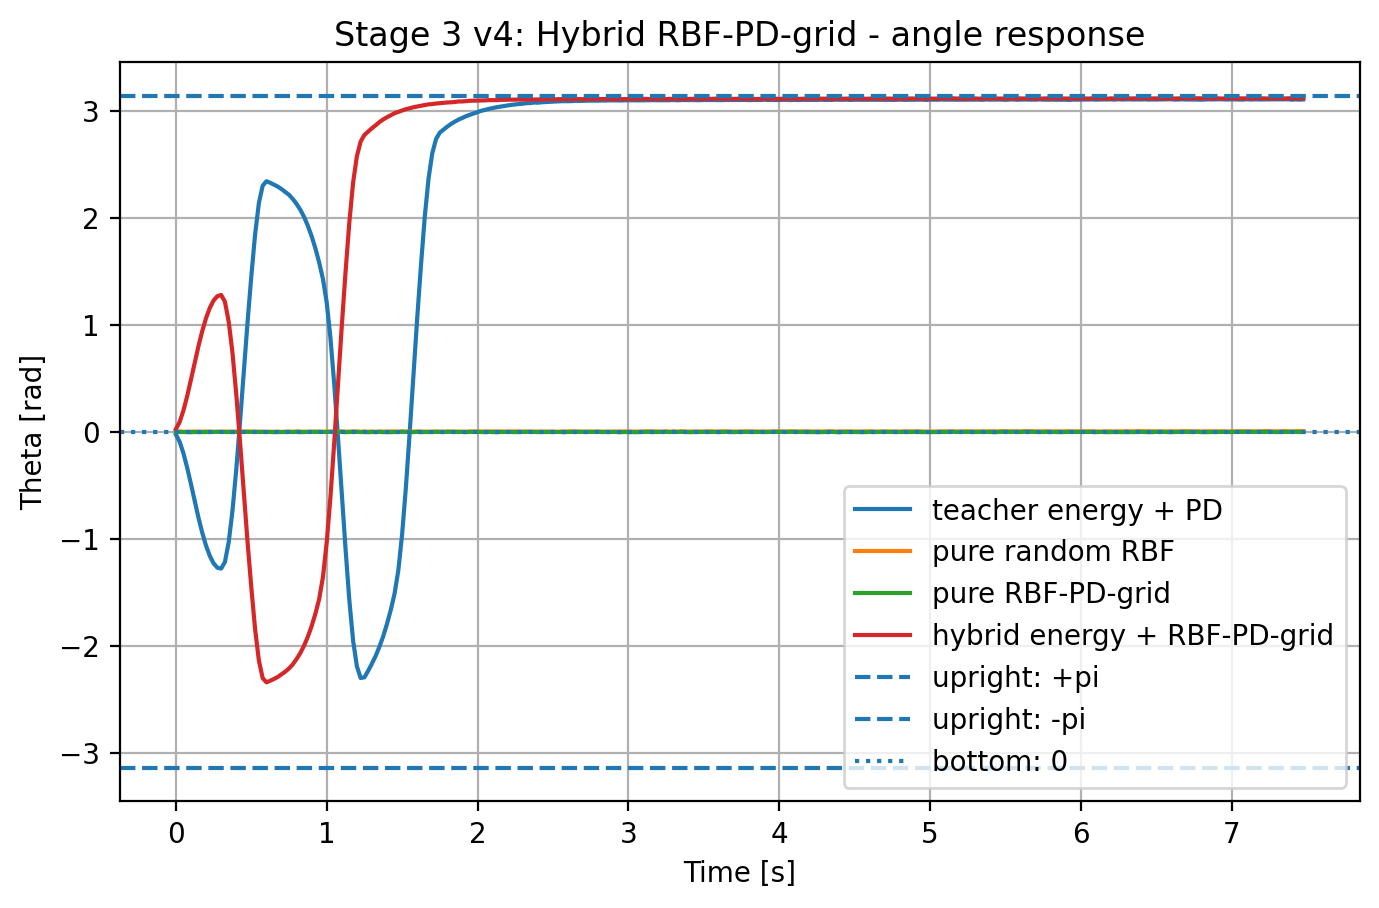
\includegraphics[width=0.85\linewidth]{figures/hybrid_rbf_pd_theta.png}
    \caption{Angle response of the initialized hybrid energy-pumping and
    RBF-PD-grid controller.}
    \label{fig:hybrid_initial_angle}
\end{figure}



\subsubsection{Simulator-Based Policy Improvement}

After the initialized hybrid controller achieved successful swing-up in
simulation, simulator-based policy improvement was applied to refine its
high-level behavior. Instead of optimizing all RBF weights, only four
hybrid-level parameters were tuned:
\begin{equation}
    p =
    \begin{bmatrix}
        \epsilon &
        g_{\mathrm{RBF}} &
        a_{\mathrm{energy}} &
        a_{\mathrm{kick}}
    \end{bmatrix}^{\top},
\label{eq:hybrid_parameters}
\end{equation}
where \(\epsilon\) is the switching threshold, \(g_{\mathrm{RBF}}\) is the RBF
stabilizer gain, \(a_{\mathrm{energy}}\) is the energy-pumping amplitude, and
\(a_{\mathrm{kick}}\) is the initial kick amplitude. This keeps the optimization
low-dimensional while preserving the PD-initialized RBF stabilizer.

The initial parameter vector was
\begin{equation}
    p_0 =
    \begin{bmatrix}
        0.45 & 1.00 & 3.00 & 2.50
    \end{bmatrix}^{\top}.
\label{eq:hybrid_initial_parameters}
\end{equation}
The parameters were optimized in the simulator using a rollout-based objective
that penalized final angle error, angular velocity, input effort, and input
saturation, while rewarding successful upright stabilization. Differential
evolution was used for global search, followed by Powell optimization for local
refinement \cite{storn1997differential,powell1964efficient}. The optimized parameter vector was
\begin{equation}
    p^{\star} =
    \begin{bmatrix}
        0.5785 & 1.3974 & 2.7481 & 2.3309
    \end{bmatrix}^{\top}.
\label{eq:hybrid_optimized_parameters}
\end{equation}
Compared with the initial controller, the optimized policy switches earlier to
the RBF stabilizer, applies a stronger local stabilizing gain, and uses smaller
energy-pumping and kick amplitudes. This improves stabilization accuracy while
reducing input saturation.

\begin{table}[htbp]
    \caption{Simulator-based policy optimization results for the hybrid
    controller.}
    \centering
    \begin{tabular}{lcc}
        \toprule
        Metric & Initial & Optimized \\
        \midrule
        Final error [rad] & $-0.025$ & $-0.011$ \\
        Min. abs. error [rad] & $0.021$ & $0.011$ \\
        Last-window error [rad] & $0.025$ & $0.013$ \\
        Saturation ratio & $0.233$ & $0.000$ \\
        Upright ratio & $0.753$ & $0.847$ \\
        RBF mode ratio & $0.767$ & $0.867$ \\
        \bottomrule
    \end{tabular}
    \label{tab:hybrid_optimization}
\end{table}

As shown in Table~\ref{tab:hybrid_optimization}, the optimized hybrid policy
reduced the last-window error from \(0.025\) rad to \(0.013\) rad and decreased
the saturation ratio from \(0.233\) to \(0.000\). Thus, the simulator-based
policy improvement made the controller more accurate and less dependent on
saturated voltage input.


\subsubsection{Robustness Evaluation}

The optimized hybrid policy was evaluated over 50 random simulation seeds to
test whether the controller generalizes to different initial perturbations and
stochastic simulation conditions. The controller parameters were fixed during
this evaluation, and no further training or optimization was performed. A
rollout was classified as successful if
\begin{equation}
\begin{aligned}
    e_{\mathrm{last}} < 0.10
    \quad \mathrm{and} \quad
    r_{\mathrm{upright}} > 0.70.
\end{aligned}
\label{eq:hybrid_success_condition}
\end{equation}

Table~\ref{tab:hybrid_robustness} summarizes the robustness results. The
optimized hybrid policy achieved a $100\%$ success rate over all 50 rollouts.
The mean last-window error was only $0.0129$ rad, and the last-window angular
velocity was $0.0011$ rad/s, indicating stable upright behavior rather than a
short pass through the target. The saturation ratio was zero for all rollouts,
and the maximum absolute input was $2.7481$ V, which remains below the
\(\pm 3\) V voltage limit.

\begin{table}[htbp]
    \caption{Robustness evaluation of the optimized hybrid policy over 50
    random seeds.}
    \centering
    \begin{tabular}{lc}
        \toprule
        Metric & Value \\
        \midrule
        Final error [rad] & $0.0010 \pm 0.0118$ \\
        Min. abs. error [rad] & $0.0099 \pm 0.0005$ \\
        Last-window error [rad] & $0.0129 \pm 0.0002$ \\
        Last-window $|\omega|$ [rad/s] & $0.0011 \pm 0.0001$ \\
        Saturation ratio & $0.0000 \pm 0.0000$ \\
        Upright ratio & $0.8475 \pm 0.0015$ \\
        RBF mode ratio & $0.8667 \pm 0.0000$ \\
        Mean absolute input [V] & $0.6298 \pm 0.0018$ \\
        Maximum absolute input [V] & $2.7481 \pm 0.0000$ \\
        \bottomrule
    \end{tabular}
    \label{tab:hybrid_robustness}
\end{table}

Overall, the optimized hybrid controller achieved reliable swing-up and
stabilization with small steady-state error and no input saturation in the
multi-seed robustness test. This shows that the hybrid RBF-based policy
improvement method provides a robust continuous-control alternative to the DQN
controller in simulation.


\subsection{Comparison of the Two Controllers}

Both the DQN controller and the optimized hybrid RBF controller achieved
successful swing-up and upright stabilization in simulation, but they use
different learning principles. The DQN controller is a value-based RL method
that learns an action-value function directly from simulator interaction. In
contrast, the hybrid RBF controller combines a physically motivated
energy-pumping law, a learned local RBF stabilizer, and simulator-based tuning
of a small number of high-level parameters \cite{course5sc28}.

\begin{table}[htbp]
    \caption{Comparison of the DQN controller and the optimized hybrid RBF
    controller in multi-seed simulation evaluation.}
    \centering
    \begin{tabular}{lcc}
        \toprule
        Metric & DQN & Hybrid RBF \\
        \midrule
        Evaluation seeds & $20$ & $50$ \\
        Success rate & $1.000$ & $1.000$ \\
        Final error [rad] & $0.0326 \pm 0.0068$ & $0.0010 \pm 0.0118$ \\
        Last-window error [rad] & $0.0317$ & $0.0129$ \\
        Last-window $|\omega|$ [rad/s] & $0.0014$ & $0.0011$ \\
        Upright ratio & $0.9233$ & $0.8475$ \\
        Saturation ratio & $0.0733$ & $0.0000$ \\
        Maximum input [V] & -- & $2.7481$ \\
        \bottomrule
    \end{tabular}
    \label{tab:controller_comparison}
\end{table}

As shown in Table~\ref{tab:controller_comparison}, both controllers reached a
success rate of \(1.000\). The DQN policy spent a larger fraction of the rollout
inside the upright region, with an upright ratio of \(0.9233\). However, the
optimized hybrid RBF controller achieved a smaller last-window error
(\(0.0129\) rad compared with \(0.0317\) rad) and completely avoided input
saturation in the robustness test. This indicates that the hybrid controller
provided more accurate final stabilization and less aggressive input behavior.

The main advantage of the DQN controller is that it learns the swing-up policy
directly from interaction data without an explicitly designed energy-pumping
law. However, it requires a discrete voltage action set and depends strongly on
reward shaping and training stability. The hybrid RBF controller uses more
prior knowledge, including the energy-pumping structure, switching logic, and
PD-based local initialization. Its advantage is that this structure reduces the
learning difficulty and gives smoother, more input-efficient control in
simulation. Therefore, the DQN controller is the clearer Q-learning-based
solution, while the optimized hybrid RBF controller gives the best simulated
steady-state accuracy and input behavior for the swing-up stabilization task.



\section{Reference Tracking}

The final part of the assignment requires a single policy that can both swing up
the disk from the downward position and track a reference motion around the
upright position \cite{assignment5sc28}. To address this task, the fixed-target DQN controller was
extended to a reference-conditioned DQN policy. The same learned policy is used
for both swing-up and tracking, rather than switching between separately trained
controllers. The wrapped tracking error is defined as
\begin{equation}
    e_{\mathrm{trk},k}
    =
    \mathrm{wrap}(\theta_k-\theta_{\mathrm{ref},k}),
\label{eq:tracking_error}
\end{equation}
and the input is constrained by \(u_k\in[-3,3]\) V.

The reference-conditioned DQN follows the same value-based learning principle
as the fixed-target DQN, but the state and reward are modified so that the
policy can react to the provided reference trajectory. The reward penalizes the
wrapped tracking error, excessive angular velocity, and unnecessary input
effort, while still encouraging successful swing-up. During training,
\(\epsilon\)-greedy exploration, experience replay, and a target network were
used as in the fixed-target DQN controller \cite{course5sc28,mnih2015dqn}. The increasing training return and
decreasing last-window tracking error indicated that the policy learned the
combined swing-up and tracking task.

After training, the best checkpoint was evaluated using the greedy policy.
Figure~\ref{fig:ref_dqn_eval} shows the measured angle, reference trajectory,
and wrapped tracking error. The disk is first swung up from the downward
position. During this initial transient, the tracking error is large because
the disk is still far from the reference. After the swing-up phase, the angle
approaches the reference around the upright position and the wrapped tracking
error remains close to zero.

\begin{figure}[H]
    \centering
    \begin{subfigure}[t]{0.48\linewidth}
        \centering
        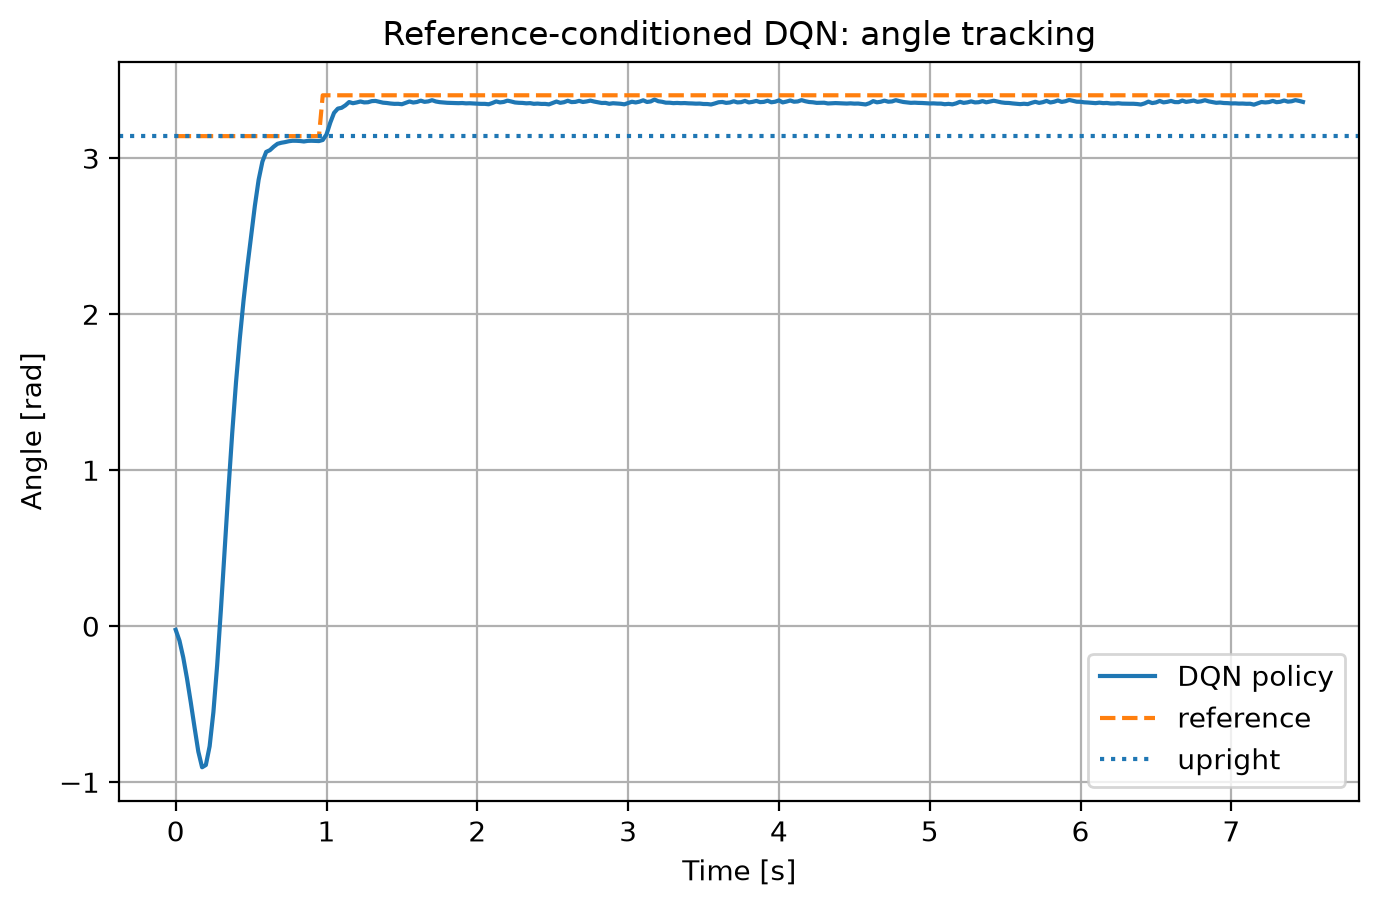
\includegraphics[width=\linewidth]{figures/ref_dqn_eval_best_theta_ref.png}
        \caption{Angle and reference.}
        \label{fig:ref_dqn_theta_ref}
    \end{subfigure}
    \hfill
    \begin{subfigure}[t]{0.48\linewidth}
        \centering
        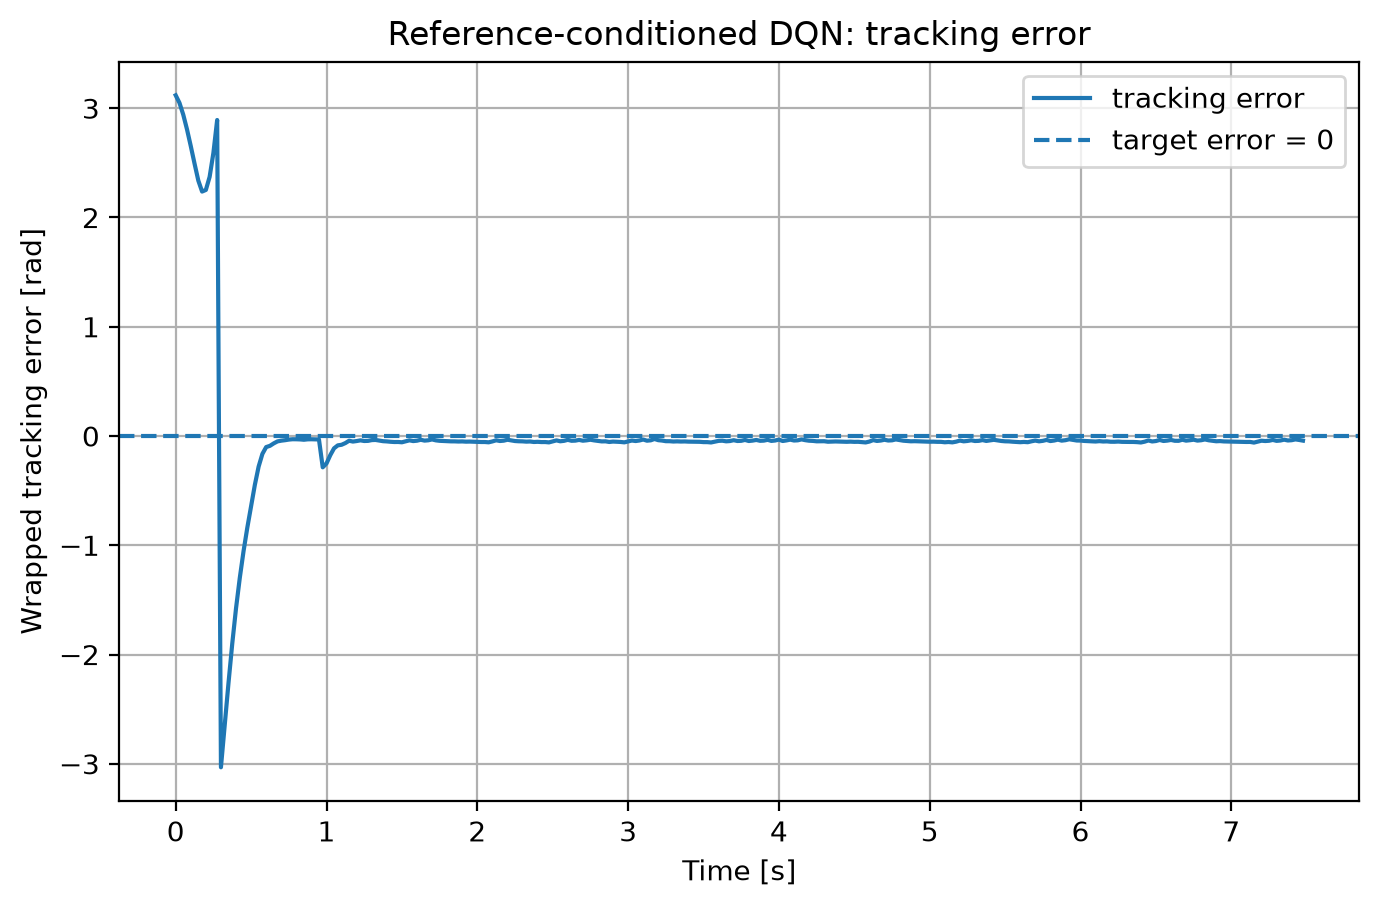
\includegraphics[width=\linewidth]{figures/ref_dqn_eval_best_error.png}
        \caption{Wrapped tracking error.}
        \label{fig:ref_dqn_tracking_error}
    \end{subfigure}
    \caption{Evaluation of the reference-conditioned DQN policy. The policy
    first swings up the disk and then tracks the reference around the upright
    region.}
    \label{fig:ref_dqn_eval}
\end{figure}

The policy was further evaluated over 20 random seeds. The results are
summarized in Table~\ref{tab:ref_dqn_results}. The reference-conditioned DQN
achieved a success rate of \(1.000\). The mean final tracking error was
\(-0.0254\) rad, the mean last-window tracking error was \(0.0310\) rad, and
the tracking ratio was \(0.9192\). These results show that the policy
consistently tracks the reference after the swing-up transient.

\begin{table}[htbp]
    \caption{Multi-seed evaluation performance of the reference-conditioned
    DQN policy.}
    \centering
    \begin{tabular}{lc}
        \toprule
        Metric & Value \\
        \midrule
        Final tracking error [rad] & $-0.0254 \pm 0.0175$ \\
        Min. abs. error [rad] & $0.0090 \pm 0.0127$ \\
        Mean abs. error [rad] & $0.1882 \pm 0.0125$ \\
        Last-window tracking error [rad] & $0.0310 \pm 0.0160$ \\
        Last-window $|\omega|$ [rad/s] & $0.3093 \pm 0.1156$ \\
        Tracking ratio & $0.9192 \pm 0.0041$ \\
        Saturation ratio & $0.1553 \pm 0.0979$ \\
        Maximum input [V] & $3.0000 \pm 0.0000$ \\
        Return & $1372.2714 \pm 6.4402$ \\
        \bottomrule
    \end{tabular}
    \label{tab:ref_dqn_results}
\end{table}

The full-rollout mean absolute error is larger than the last-window tracking
error because it includes the initial swing-up transient. Therefore, the
last-window error better reflects the steady-state tracking performance after
the disk has reached the upright region. The saturation ratio was \(0.1553\),
and the maximum input magnitude was \(3.0\) V, confirming that the voltage
constraint was satisfied but that the discrete DQN policy still used saturated
actions during part of the rollout.

Overall, the reference-conditioned DQN successfully extends the fixed-target
swing-up controller to reference tracking around the upright position using a
single learned policy. The main limitation is the switching input caused by the
discrete action representation. In addition, the current evaluation is based on
the tested reference trajectory; further tests with multiple reference signals
over the full \(\pm 15^\circ\) range would provide a more complete assessment.


\section{Real-Setup Experiments}

\subsection{Real-Setup Test Plan}

After validating the controllers in simulation, preliminary real-setup
experiments were carried out to investigate their transfer to the physical
unbalanced-disk system. The purpose of these tests was not to obtain a fully
optimized hardware demonstration, but to identify practical effects that are
not present in simulation, such as sensor bias, voltage limitations,
state-estimation errors, and safety constraints.

The real setup was accessed through
\texttt{gym\_unbalanced\_disk.UnbalancedDisk\_exp}. The sampling time was
\begin{equation}
    T_s = 0.025~\mathrm{s}.
\label{eq:real_sampling_time}
\end{equation}
The hardware interface allows the assignment voltage range
\begin{equation}
    u_k \in [-3,3]~\mathrm{V}.
\label{eq:real_voltage_range}
\end{equation}
However, conservative voltage limits were used during the first hardware tests
for safety. In the DQN safe deployment test, the applied input was clipped to
\begin{equation}
    u_k \in [-2,2]~\mathrm{V},
\label{eq:real_dqn_safe_voltage}
\end{equation}
which made the real experiment more restrictive than the simulation training
environment.

A practical issue was the angular velocity measurement. The raw velocity signal
showed noticeable bias and noise, so it was recorded for analysis but not used
directly for feedback. Instead, the controller used a filtered finite-difference
estimate from the measured angle,
\begin{equation}
\begin{aligned}
    \omega_{\mathrm{est},k}
    =
    \alpha \omega_{\mathrm{est},k-1}
    +
    (1-\alpha)
    \frac{\mathrm{wrap}(\theta_k-\theta_{k-1})}{T_s}.
\end{aligned}
\label{eq:real_velocity_estimate}
\end{equation}
The filter coefficient was set to \(\alpha=0.80\).
Safety checks were included to stop the experiment if the unwrapped angle or
estimated angular velocity exceeded predefined limits. The logged signals
included the measured angle, estimated velocity, raw velocity, applied voltage,
wrapped upright error, and controller action or mode information.

Therefore, the real-setup experiments should be interpreted as safe preliminary
deployment tests. Their main role is to evaluate simulation-to-real transfer
and identify the practical limitations that prevent direct deployment of the
simulation-trained controllers.



\subsection{Real-Setup DQN Safe Deployment}

The first controller tested on the real setup was the DQN swing-up policy
trained in simulation. The same sine-cosine state representation was used, but
the angular velocity was replaced by the filtered estimate
\(\omega_{\mathrm{est}}\) obtained from the measured angle. The original DQN
action set contained voltages up to \(\pm 3\) V, but during the first safe
hardware deployment the selected action was clipped to \([-2,2]\) V. This
reduced the risk to the setup, but also made the real experiment more
restrictive than the simulation training environment.

Figure~\ref{fig:real_dqn_theta_input} shows the measured angle and applied
input during the real DQN safe test. The disk moved only to a small offset from
the downward equilibrium and did not approach the upright position
\(\theta=\pm\pi\). At the same time, the applied input remained close to the
positive safety limit of \(+2\) V for most of the rollout. This indicates that
the policy repeatedly selected a large positive action that was clipped by the
real-system safety bound. As a result, the controller behaved almost like a
constant-voltage input rather than a feedback policy that successfully adapted
during swing-up.

\begin{figure}[H]
    \centering
    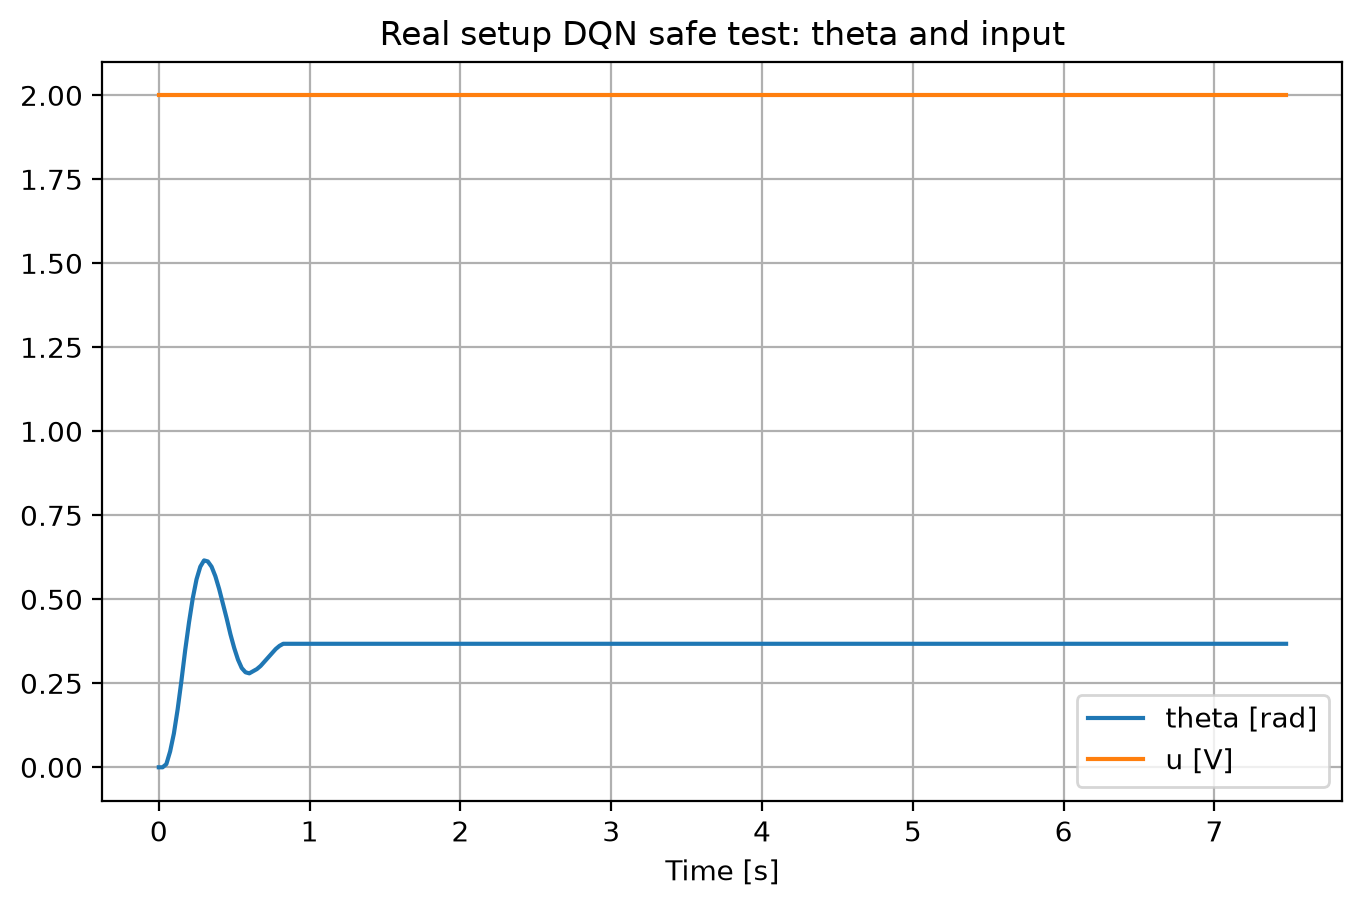
\includegraphics[width=0.75\linewidth]{figures/real_dqn_safe_theta_input.png}
    \caption{Measured angle and applied input during the real-setup DQN safe
    deployment test. Input remains close to the \(+2\) V safety limit, while
    the disk fails to reach the upright position.}
    \label{fig:real_dqn_theta_input}
\end{figure}

The result should therefore be interpreted as an unsuccessful direct transfer
from simulation to hardware. The conservative voltage clipping is one important
reason: the DQN was trained with actions up to \(\pm 3\) V, while the real test
allowed only \(\pm 2\) V, reducing the available swing-up energy. In addition,
the real setup differs from the simulator because of friction, delay, actuator
behavior, sensor noise, and velocity-estimation errors. The raw angular
velocity measurement showed bias and noise, so the controller used an
angle-based filtered estimate instead. This changed the state distribution seen
by the DQN policy and likely contributed to the nearly constant-action behavior
observed in the real experiment.


\subsection{Real-Setup Hybrid RBF Policy Test}

The second controller tested on the real setup was the optimized hybrid
energy-pumping and RBF policy. The real implementation used three modes:
Energy, Brake, and RBF. The Energy mode was used for swing-up energy injection,
the Brake mode was added to reduce excessive angular velocity near the upright
region, and the RBF mode was used for local stabilization. For safety, the
voltage limits were set to \(\pm 2.0\) V in Energy mode, \(\pm 0.5\) V in Brake
mode, and \(\pm 1.2\) V in RBF mode. As in the DQN real-setup test, the raw
angular velocity was recorded only for analysis, while the feedback velocity
was estimated from the measured angle because of bias and noise in the raw
sensor signal.

Figure~\ref{fig:real_hybrid_theta} shows the measured angle during the real
hybrid RBF test. Compared with the real DQN safe deployment, the hybrid
controller generated much larger disk motion and approached the upright region
several times. This shows that the energy-pumping part transferred better to
the physical setup. However, the disk still continued to oscillate with large
amplitude and did not achieve sustained upright stabilization. Thus, the real
hybrid policy achieved partial transfer: it could generate swing-up motion, but
the capture and local stabilization phase was not robust enough on the real
setup.

\begin{figure}[H]
    \centering
    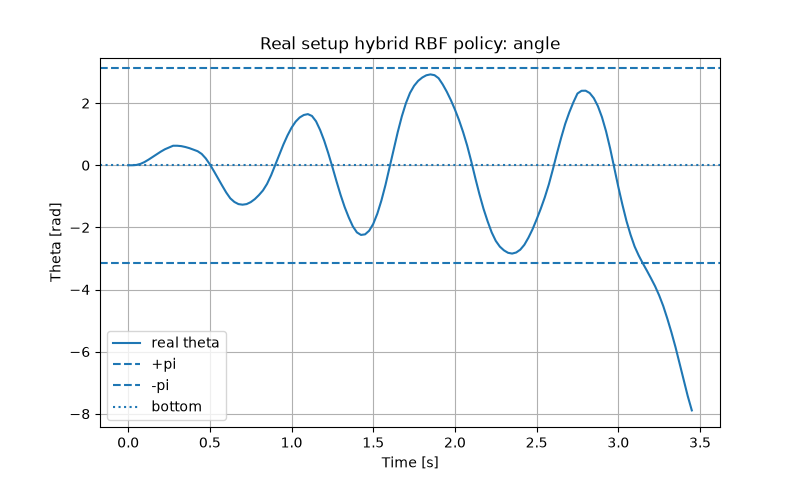
\includegraphics[width=0.75\linewidth]{figures/real_hybrid_rbf_theta.png}
    \caption{Angle response of the real-setup hybrid RBF policy. The controller
    approaches the upright region but does not achieve sustained stabilization.}
    \label{fig:real_hybrid_theta}
\end{figure}

The input and mode behavior in Fig.~\ref{fig:real_hybrid_input_mode} explain
the failed capture. The input frequently reaches the Energy-mode limits,
showing that the controller relies mainly on energy pumping. Meanwhile, the
mode signal shows that Brake and RBF modes are only activated briefly near the
upright region. Therefore, the main issue is not the lack of swing-up energy,
but the inability to remain in the local stabilization modes long enough to
capture the disk near the upright equilibrium.

\begin{figure}[H]
    \centering
    \begin{subfigure}[t]{0.48\linewidth}
        \centering
        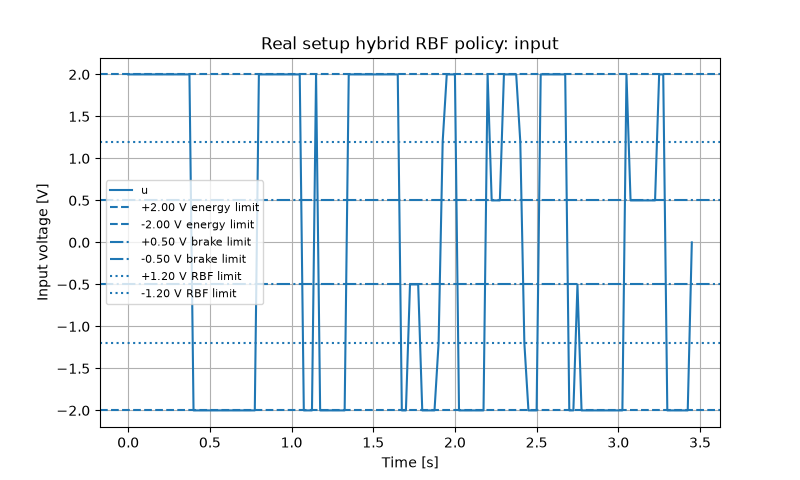
\includegraphics[width=\linewidth]{figures/real_hybrid_rbf_input.png}
        \caption{Applied input voltage.}
        \label{fig:real_hybrid_input}
    \end{subfigure}
    \hfill
    \begin{subfigure}[t]{0.49\linewidth}
        \centering
        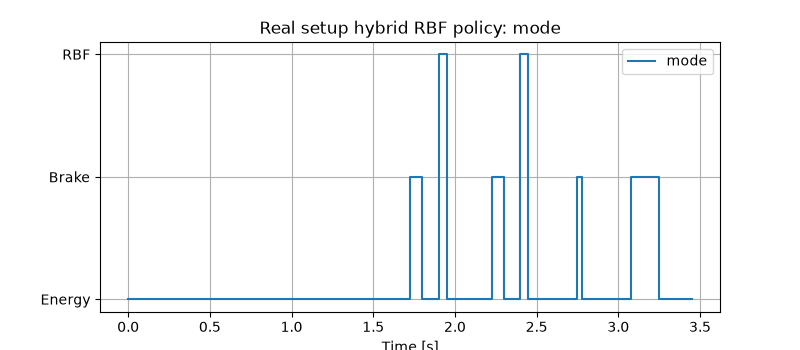
\includegraphics[width=\linewidth]{figures/real_hybrid_rbf_mode.png}
        \caption{Control mode.}
        \label{fig:real_hybrid_mode}
    \end{subfigure}
    \caption{Input and mode behavior of the real-setup hybrid RBF policy.}
    \label{fig:real_hybrid_input_mode}
\end{figure}

This behavior is likely caused by the limited authority of the Brake and RBF
modes and the sensitivity of the switching logic to velocity estimation, noise,
and real-system mismatch. Since the switch to Brake or RBF mode depends on the
wrapped upright error and estimated angular velocity, an inaccurate or delayed
velocity estimate can cause the controller to enter the local stabilization
region too early, too late, or for too short a time. Overall, the real hybrid
RBF controller transferred better than the real DQN policy in terms of energy
generation, but reliable upright capture still requires further real-system
tuning of the switching conditions and local stabilizer.


\subsection{Discussion of Simulation-to-Real Gap}

The real setup experiments revealed a clear simulation-to-real gap. In
simulation, both the DQN controller and the optimized hybrid RBF controller
achieved successful swing-up and stabilization. On the physical setup, however,
the DQN controller did not generate sufficient swing-up motion, while the
hybrid RBF controller produced large oscillations but failed to reliably capture
and stabilize the disk near the upright position.

For the DQN controller, the main issue was the mismatch between the simulation
training conditions and the safe hardware deployment. The policy was trained
with actions up to \(\pm 3\) V, but the real experiment clipped the applied
voltage to \(\pm 2\) V. This reduced the available swing-up energy and caused
the input to remain close to the positive safety limit without producing enough
motion to reach the upright region. In addition, the real setup used a filtered
angle-based velocity estimate instead of the clean simulated velocity, which
changed the state distribution seen by the neural network.

The hybrid RBF controller showed better partial transfer because its
energy-pumping component could excite the disk and bring it close to the
upright region. However, the capture phase was not robust enough. The Brake and
RBF modes had smaller safety-limited voltages, and the switching logic depended
on the estimated angular velocity. Therefore, velocity-estimation errors,
sensor noise, delay, friction, and actuator mismatch could cause the controller
to enter the local stabilization modes at unsuitable times or for too short a
duration.

Overall, the real experiments show that successful simulated swing-up does not
guarantee direct hardware transfer. The DQN test highlights the sensitivity of
learned value-based policies to voltage limits and state-distribution changes,
while the hybrid RBF test shows that physical insight improves energy
generation but does not by itself guarantee robust capture. Future work should
focus on safer but less restrictive voltage scheduling, better angular-velocity
calibration, real-setup retuning of switching thresholds and local gains, and
training with domain randomization or real-system data.


\section{Discussion}

\subsection{Model Comparison}

Table~\ref{tab:ann_gp_comparison} compares the best ANN results with the final GP result.
For the ANN, the best prediction result was obtained with the GRU model, while the best simulation result was obtained with the LSTM model.
The GP model was a sparse delta-output GP-NARX model.

\begin{table}[htbp]
\caption{Best ANN and GP modelling results. The ANN values are the best ANN results per task on the held-out test split, while the GP values are validation results from the GP pipeline.}
\centering
\begin{tabular}{lcc}
\toprule
Model & Prediction RMSE & Simulation RMSE \\
\midrule
Best ANN & 0.202 deg & 1.893 deg \\
Best GP & 0.164 deg & 1.461 deg \\
\bottomrule
\end{tabular}
\label{tab:ann_gp_comparison}
\end{table}

The GP model obtained the lowest recorded prediction and simulation RMSE.
Relative to the best ANN results, it reduced prediction RMSE by about
\(19\%\) and simulation RMSE by about \(23\%\). The ``Best ANN'' row combines
the GRU prediction result and the LSTM simulation result, since these were the
best ANN models for the two tasks.

The ANN and GP approaches also have different practical advantages.
The GP provides a probabilistic framework and achieved high accuracy
with the available dataset, while recurrent neural networks can be
scaled more easily to substantially larger datasets and more complex
architectures. Therefore, the lower GP errors in this project should not
be interpreted as a general conclusion that GP models are always more
accurate than ANN models. They only show that the final sparse GP model
performed best among the configurations tested here.

A strictly fair numerical comparison would require the ANN and GP
models to use exactly the same held-out samples, preprocessing steps,
simulation initialization, simulation horizon, and error definition.
In this project, the ANN values were computed on the ANN held-out test
split, while the GP values were reported from the GP validation
pipeline. The comparison in Table~\ref{tab:ann_gp_comparison} should
therefore be interpreted as a practical comparison of the final
recorded models, not as a perfectly controlled benchmark.


\subsection{Controller Discussion}

This project evaluated three learning-based control results for the unbalanced
disk: a DQN swing-up controller, an optimized hybrid RBF swing-up controller,
and a reference-conditioned DQN tracking controller. In simulation, all three
controllers achieved the intended task. The fixed-target DQN reached a success
rate of \(1.000\) over 20 seeds, with a last-window angle error of
\(0.0317\) rad. The optimized hybrid RBF controller also achieved a success
rate of \(1.000\), with a smaller last-window error of \(0.0129\) rad and zero
input saturation over 50 seeds. For the reference-tracking task, the
reference-conditioned DQN achieved a success rate of \(1.000\), a last-window
tracking error of \(0.0310\) rad, and a tracking ratio of \(0.9192\).

The DQN is the clearest Q-learning-based solution, but its discrete action set
makes the input less smooth and its performance depends on reward shaping. The
hybrid RBF controller uses more prior structure: energy-pumping for swing-up
and an RBF policy for local stabilization. This improves simulated accuracy and
input behavior, but it is not a fully end-to-end reinforcement learning method.

The real setup experiments showed that good simulation performance did not
directly guarantee successful hardware transfer. The DQN safe deployment did
not swing up the disk, mainly because the real test used a conservative
\(\pm 2\) V voltage limit instead of the \(\pm 3\) V action range used during
training, and because the measured real-state information differed from the
simulation state. The hybrid RBF controller transferred better in the
energy-building phase and brought the disk close to the upright region several
times, but it still failed to achieve reliable capture and sustained
stabilization. This indicates that the local stabilization and switching logic
were not robust enough under real-system conditions.

Overall, value-based learning and hybrid policy improvement both solved the
simulated swing-up task, and the reference-conditioned DQN extended the task to
tracking. The main remaining limitation is the simulation-to-real gap.



\subsection{Limitations}

The main project limitation is that the search over models and
controllers was limited by time. The selected ANN, GP, and control
methods are therefore the best among the configurations tested in this
project, but they are not guaranteed to be globally optimal.

The conclusions also depend on the available data and simulation
conditions. The modelling data only cover a finite range of voltage
signals and disk motions, so performance may change for trajectories
outside this range. Similarly, policies that work well in simulation
may behave differently on the real setup because of friction, delay,
sensor noise, saturation, or mismatch between the simulator and the
physical system.

The comparison between methods should also be interpreted carefully.
The ANN and GP models were both tested on prediction and simulation
tasks, but they were not tuned with exactly the same number of trials or
the same type of hyperparameters. The true measured outputs for the
hidden benchmark tests were not available during development, so the
final hidden-test files could only be checked for the required format
before being evaluated by the course staff.

\section{Conclusion}

This project studied both data-driven modelling and learning-based control of
the unbalanced disk. For the modelling task, all models used the required input
and output signals: motor voltage and measured disk angle. Among the ANN
models, the GRU gave the best one-step prediction result and the LSTM gave the
best free-run simulation result. The sparse delta-output GP-NARX model achieved
the lowest recorded modelling errors, showing that the selected GP structure
was well suited to the available identification data.

For the control task, the DQN controller successfully learned swing-up and
upright stabilization in simulation. The reference-conditioned DQN also showed
that one learned policy can combine swing-up with tracking around the upright
position. The optimized hybrid RBF controller gave the best simulated
steady-state accuracy and avoided input saturation in the robustness test.
However, the real setup experiments showed that good simulation performance did
not directly transfer to hardware. The DQN was too limited by the conservative
voltage bound, while the hybrid controller transferred the swing-up energy
building better but did not reliably capture the disk near upright. The main
future improvements are real-system retuning, better angular-velocity
estimation, and training with more uncertainty or real-system data.

\bibliographystyle{IEEEtran}
\bibliography{references}

\end{document}
